%% Класс-заглушка для компилируемого черновика: используемые команды (\email, \orcid,
%% \affiliation, \teaserfigure, \keywords, \Description, acks, ACM-Reference-Format) взяты из acmart.
%% Финальный класс будет выбран под конкретную площадку.
\documentclass[sigconf,nonacm]{acmart}

%%
%% \BibTeX command to typeset BibTeX logo in the docs
\AtBeginDocument{%
    \providecommand\BibTeX{{%
        Bib\TeX}}}

\usepackage[T1,T2A]{fontenc}
\usepackage[utf8]{inputenc}
\usepackage[russian,english]{babel}
\usepackage{algorithm}
\usepackage{algorithmic}
\usepackage{graphicx}
\usepackage{amssymb}
\usepackage{textcomp}
\usepackage{booktabs}
\usepackage{amsopn}


\begin{document}
    \title{IduEdu: A Pipeline for Multimodal Urban Graphs Construction and Large-Scale Accessibility Analysis}


    \author{Danila Oleynikov}
    \email{ddonnyy@itmo.ru}
    \orcid{0009-0002-7881-1543}
    \affiliation{%
        \institution{ITMO University}
        \city{Saint-Petersburg}
        \country{Russia}
    }



    \begin{abstract}

        Open geospatial data provides the foundation for reproducible and accessible urban analysis; however,
        its practical use requires efficient open-source tools capable of handling large-scale transportation networks.
        This paper presents IduEdu—an open-source Python library and pipeline for multimodal urban graph construction,
        including street network extraction, static public transport graph construction, pedestrian–transport graph
        integration, and scalable computation of origin–destination (OD) matrices.
        IduEdu is built on UrbanGraph, a tabular GeoDataFrame-native graph representation in which the spatial and the computational forms of
        the network coincide, eliminating format conversions across the entire pipeline.
        Experimental evaluation on large-city data shows that IduEdu builds street graphs $5$--$9\times$ faster than OSMnx,
        while producing an in-memory graph representation about an order of magnitude smaller.
        For large-scale origin--destination (OD) computation, the combination of adaptive graph reversal and a
        time/distance cutoff lets IduEdu match or outperform optimized C/C++ graph libraries (NetworKit, igraph) on
        batch-accessibility workloads, without any graph-format conversion step.
        Correctness is verified against a NetworkX reference: reachability sets coincide exactly and accessibility values
        agree within $3\cdot10^{-4}$~min, while the total street-network length matches OSMnx within ${\approx}1\%$.

    \end{abstract}


    \keywords{urban networks, multimodal graphs, OpenStreetMap, accessibility analysis, origin--destination matrices, open-source software}

    \begin{teaserfigure}
        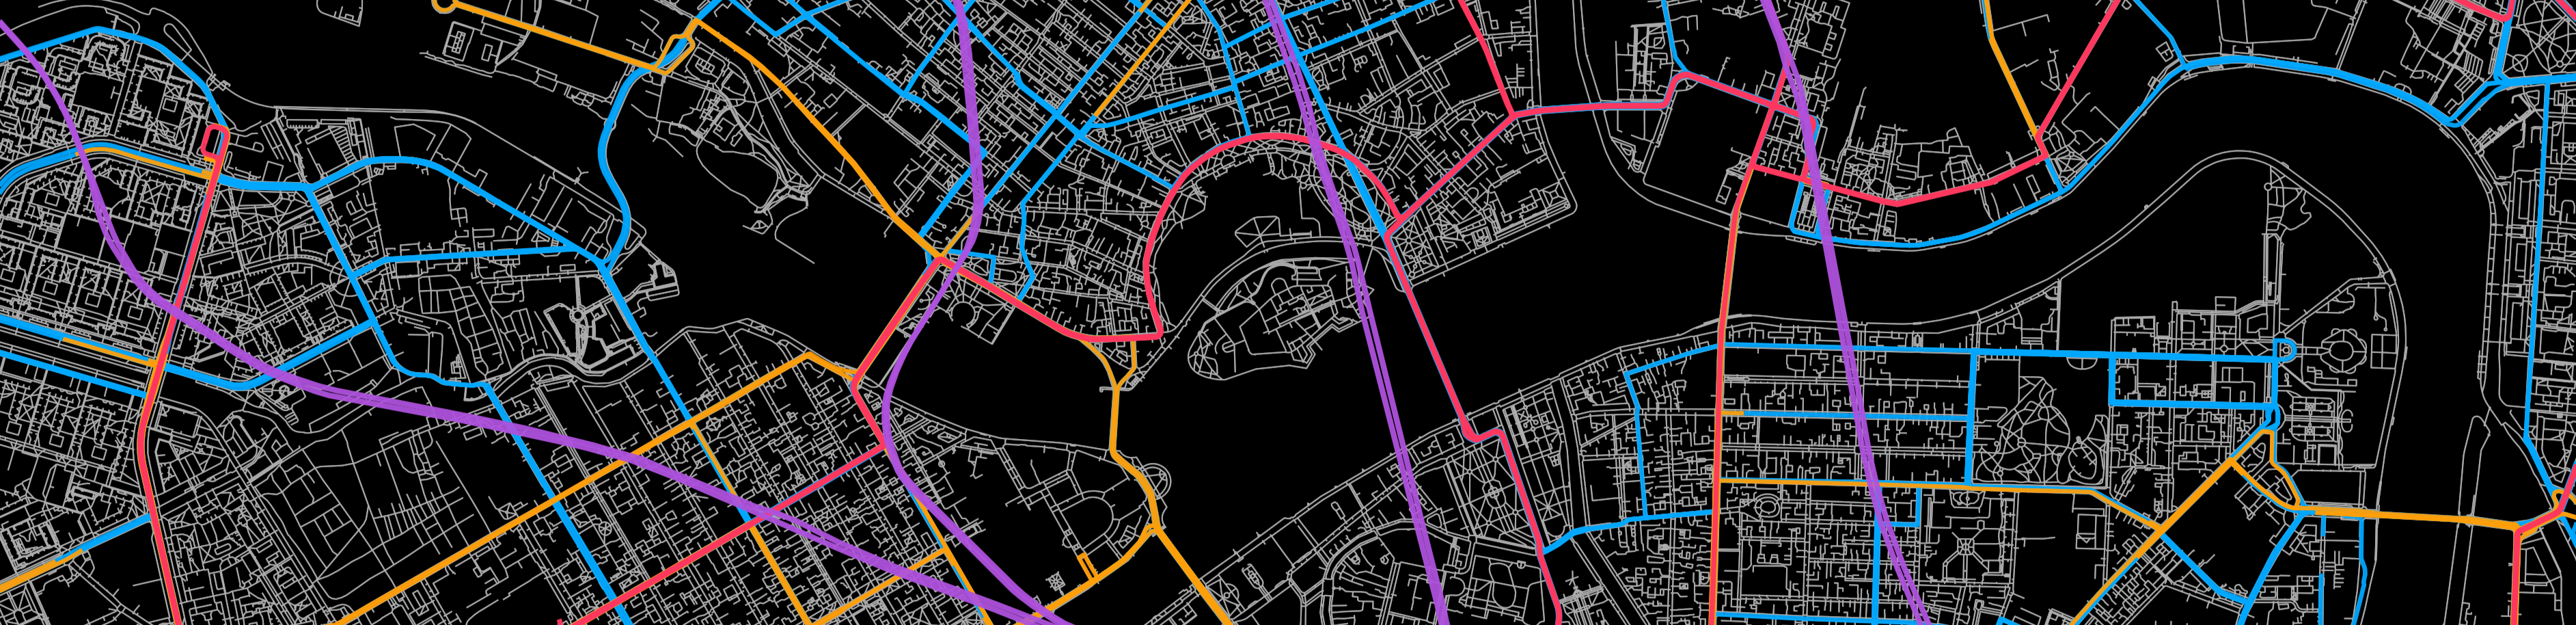
\includegraphics[width=\textwidth]{figures/teaser_figure}
        \caption{Multi-modal network combining pedestrian and public transport graphs extracted from OpenStreetMap with IduEdu.}
        \Description{Pedestrian and public transport networks extracted from OpenStreetMap and visualized on a dark background.
        Walking edges are shown in light gray; public transport modes are highlighted with distinct colors.}
        \label{fig:teaser}
    \end{teaserfigure}


    \maketitle


    \section{Introduction}
    Городские транспортные системы традиционно анализируются с использованием пространственных графов и матриц
    корреспонденций (origin–destination, OD), которые служат базовыми инструментами для оценки доступности, связности
    и городской мобильности.
    Развитие открытых геоданных, в частности проекта OpenStreetMap (OSM), сделало возможным проведение такой аналитики на
    уровне целых городов широкому кругу исследователей.
    Однако, несмотря на доступность данных, воспроизводимый и масштабируемый анализ мультимодальной городской мобильности
    по-прежнему остаётся методологически сложной задачей.

    Существующие open-source инструменты, как правило, охватывают лишь отдельные этапы этого процесса.
    В результате исследователи вынуждены комбинировать несколько разрозненных библиотек и форматов данных.
    Особенно проблематичной остаётся интеграция общественного транспорта и пешеходной сети в рамках единого графового представления.
    На практике полный цикл анализа включает (i) извлечение геоданных (ii) сборку пешеходного/транспортного/мультимодального
    графа и (iii) массовый расчёт показателей доступности, в том числе OD-матриц.
    Ни один из распространённых open-source инструментов не закрывает этот цикл целиком в рамках единого воспроизводимого пайплайна.
    Разрыв этого цикла имеет конкретную вычислительную цену: типовой стек «извлечение графа в NetworkX $\to$
    конвертация в специализированную библиотеку (NetworKit/igraph/graph-tool) ради ускорения массовых расчётов»
    требует смены представления графа между этапами, что расходует время и память тем сильнее, чем крупнее сеть.
    Отсюда исследовательский вопрос настоящей работы: \emph{можно ли построить единое представление городского графа,
        в котором форматы хранения (пространственный) и вычислений совпадают, и обеспечивает ли устранение конверсии
        измеримый выигрыш по времени и памяти на масштабе целого города при сохранении корректности результатов?}

    В данной работе представлен IduEdu — Python-пакет для построения и анализа мультимодальных городских графов на основе данных OpenStreetMap.
    Вклад работы состоит из четырёх частей: (i) табличное GeoDataFrame-представление городского графа \texttt{UrbanGraph},
    в котором вычислительный и пространственный форматы совпадают и конвертация между ними отсутствует по построению;
    (ii) построение статического графа общественного транспорта непосредственно из данных OSM без привлечения GTFS;
    (iii) масштабируемый расчёт OD-матриц с порогом отсечки и адаптивным разворотом графа на Numba-ядрах;
    (iv) открытый воспроизводимый набор бенчмарков, покрывающий сборку графов, мультимодальную интеграцию,
    расчёт кратчайших путей, потребление памяти и корректность результатов.


    \section{Related Work}
    \label{sec:related-work}

    \begin{table*}
        \caption{Сравнение open-source инструментов для построения пространственных и мультимодальных графов
        и расчёта матриц корреспонденций. Столбцы задают проверяемые критерии:
        \emph{Drive/Walk} — построение уличного графа из OSM; \emph{PT} — построение графа общественного транспорта;
        \emph{Graph export} — выдача явного графа, пригодного для произвольного анализа стандартными графовыми библиотеками;
        \emph{OD} — наличие API/алгоритмов расчёта матриц корреспонденций (без гарантии масштабируемости);
        \emph{Python-native} — работа целиком в Python без развёртывания внешнего сервиса.
        Обозначения: \checkmark — поддерживается; (\checkmark) — частичная поддержка;
        \texttimes — не поддерживается; ``--'' — не применимо.}
        \label{tab:tools_comparison}
        \begin{tabular}{lccccc}
            \toprule
            Tool                            & Drive/Walk & PT         & Graph export & OD           & Python-native \\
            \midrule
            OSMnx                           & \checkmark & \texttimes & \checkmark   & \texttimes   & \checkmark    \\
            Pyrosm                          & \checkmark & \texttimes & \checkmark   & \texttimes   & \checkmark    \\
            UrbanAccess + OSMnet            & \checkmark & \checkmark & (\checkmark) & (\checkmark) & \checkmark    \\
            Peartree                        & \texttimes & \checkmark & \checkmark   & \texttimes   & \checkmark    \\
            \midrule
            OSRM                            & \checkmark & \texttimes & \texttimes   & (\checkmark) & \texttimes    \\
            GraphHopper                     & \checkmark & \checkmark & \texttimes   & (\checkmark) & \texttimes    \\
            Valhalla                        & \checkmark & \checkmark & \texttimes   & (\checkmark) & \texttimes    \\
            OpenTripPlanner                 & \checkmark & \checkmark & \texttimes   & (\checkmark) & \texttimes    \\
            \midrule
            NetworkX                        & --         & --         & --           & (\checkmark) & \checkmark    \\
            NetworKit / Graph-tool / igraph & --         & --         & --           & (\checkmark) & (\checkmark)  \\
            \midrule
            \textbf{IduEdu}                 & \checkmark & \checkmark & \checkmark   & \checkmark   & \checkmark    \\
            \bottomrule
        \end{tabular}
    \end{table*}

    \subsection{Spatial Graph Construction from OpenStreetMap}
    \label{subsec:spatial-graph-construction-from-openstreetmap2}

    Исследования в области городской мобильности и транспортного моделирования широко опираются на представление уличных
    и транспортных систем в виде пространственных графов.
    Основным источником открытых данных для построения таких графов является OpenStreetMap.
    Однако экосистема инструментов для работы с OSM фрагментирована: отдельные решения ориентированы либо на извлечение уличных сетей,
    либо на серверную маршрутизацию, либо на отдельные аспекты мультимодального анализа.
    Как следствие, полный цикл анализа городской мобильности приходится собирать из разнородных инструментов, что снижает воспроизводимость.
    Таблица~\ref{tab:tools_comparison} суммирует ключевые возможности наиболее распространённых open-source решений.

    \subsection{Python Libraries for OSM Graph Extraction}
    \label{subsec:python-libraries-for-osm-graph-extraction}

    \textbf{OSMnx}~\cite{boeing2025osmnx} является одним из наиболее распространённых Python-инструментов для извлечения
    и анализа уличных графов на основе данных OpenStreetMap.
    Библиотека широко используется в исследованиях по городскому моделированию и анализу пространственных сетей~\cite{coutrot2022, nilsson2019, feng2020, liao2020}.
    OSMnx автоматизирует загрузку городских сетей через Overpass API~\cite{overpass_api} и формирует ориентированный
    мультиграф формата \texttt{networkx.MultiDiGraph}~\cite{hagberg2008networkx}, предоставляя поддерживаемый
    сообществом API с развитыми средствами визуализации, упрощения графов и базового анализа уличных сетей.
    При этом библиотека ориентирована исключительно на статические уличные сети и не поддерживает построение графов
    общественного транспорта или мультимодальных сетей.

    \textbf{Pyrosm}~\cite{pyrosm_docs} предоставляет альтернативный подход к построению уличных графов, основанный на работе
    с локальными PBF-файлами OpenStreetMap (бинарными дампами данных OSM); его реализация на Cython и Pyrobuf обеспечивает
    высокую производительность при обработке территорий масштаба города или страны.
    Библиотека поддерживает извлечение городских сетей и возвращает графы в форматах, совместимых с NetworkX~\cite{hagberg2008networkx} и другими Python-библиотеками.
    Как и OSMnx, Pyrosm ориентирован на статические уличные сети и не включает средства для моделирования общественного
    транспорта или расчёта матриц корреспонденций.

    \textbf{UrbanAccess}~\cite{blanchard2017urbanaccess} и связанная библиотека \textbf{OSMnet}~\cite{osmnet_github}
    входят в состав Urban Data Science Toolkit и строят мультимодальное пешеходно-транзитное представление на основе OSM и
    General Transit Feed Specification (GTFS)~\cite{gtfs_spec}: UrbanAccess обрабатывает GTFS-данные, OSMnet извлекает пешеходную сеть.
    Результат представлен таблицами \texttt{pandas.DataFrame}~\cite{mckinney2010pandas} и предназначен прежде всего для расчёта
    показателей доступности в \texttt{Pandana}~\cite{foti2014pandana}.
    Механизм загрузки GTFS в UrbanAccess опирается на каталог GTFS Data Exchange, не обновляемый с 2016 года,
    из-за чего многие фиды недоступны; последний релиз (0.2.2) датируется 2020 годом.

    \textbf{Peartree}~\cite{peartree_github} ориентирован на преобразование GTFS-данных в статический граф общественного
    транспорта на уровне маршрутов и остановок (в качестве пешеходного графа авторы предлагают OSMnx).
    Полученный граф в формате NetworkX отражает топологическую структуру транзитной сети и может быть объединён с пешеходными
    графами, однако библиотека не реализует собственных алгоритмов маршрутизации; последний релиз (0.6.4) датируется 2021 годом.

    \subsection{High-Performance Routing Engines}
    \label{subsec:high-performance-routing-engines}

    Отдельный класс решений составляют высокопроизводительные маршрутизаторы на базе OpenStreetMap,
    такие как OSRM\cite{osrm}, GraphHopper~\cite{graphhopper}, Valhalla~\cite{valhalla} и OpenTripPlanner~\cite{otp}.
    Эти системы ориентированы на серверную маршрутизацию и оптимизированы для быстрого ответа на запросы поиска маршрутов,
    матриц расстояний и изохрон на графах большого масштаба.
    Как правило, они развёртываются в виде автономных сервисов
    с HTTP API и используют специализированные структуры данных и индексацию, скрывая внутреннее представление графа от
    пользователя.

    GraphHopper, Valhalla и OpenTripPlanner поддерживают мультимодальные сценарии и интеграцию GTFS-данных с
    учётом расписаний, тогда как OSRM ограничен статичными дорожными сетями.
    При этом ни один из перечисленных маршрутизаторов не предоставляет явного графа в форме, пригодной для произвольного
    анализа и модификации стандартными графовыми библиотеками, а взаимодействие с ними из Python осуществляется
    исключительно через внешние API\@.

    \subsection{General-Purpose Graph Libraries}
    \label{subsec:general-purpose-graph-libraries}

    \textbf{NetworkX} - библиотека на языке Python, фактически ставшая стандартом де-факто для представления графов и
    реализации классических алгоритмов анализа сетей~\cite{hagberg2008networkx}.
    Многие инструменты извлечения графов из OSM, включая OSMnx, Pyrosm и Peartree, используют NetworkX в качестве
    внутреннего формата хранения.
    NetworkX предоставляет широкий набор алгоритмов анализа и поддерживает импорт/экспорт в распространённые форматы
    (GraphML, adjacency list, GEXF), что упрощает перенос графов в более быстрые backend'ы.
    Однако его объектное представление графа (словарь словарей Python-объектов) масштабируется на крупных сетях хуже
    C/C++-ядер как по времени, так и по памяти~\cite{staudt2016networkit, benchmark_graphtools}.


    \textbf{graph-tool~\cite{graphtool_docs}, igraph~\cite{csardi2006igraph} и NetworKit~\cite{staudt2016networkit}}
    представляют собой высокопроизводительные библиотеки для анализа графов с C/C++ ядром и Python-интерфейсом.
    Они демонстрируют значительное ускорение по сравнению с чисто Python-реализациями при работе с графами большого
    масштаба и обычно используются в комбинированных пайплайнах после извлечения графа другими инструментами.
    При этом эти библиотеки не решают задачи загрузки и сборки пространственных/транспортных графов из OSM/GTFS и не
    предоставляют единого end-to-end инструмента для построения мультимодальной сети и последующего расчёта метрик доступности.

    \subsection{IduEdu as a Unified Reproducible Pipeline}
    \label{subsec:iduedu-as-a-unified-reproducible-pipeline}

    В отличие от рассмотренных выше решений, охватывающих отдельные этапы работы с пространственными и транспортными графами,
    IduEdu реализует единый воспроизводимый Python-пайплайн для построения и анализа мультимодальных графов городской мобильности.
    Ключевое отличие подхода не в наборе поддерживаемых этапов как таковых, а в едином представлении графа, которое проходит через весь пайплайн:
    извлечение уличной сети, построение статического графа общественного транспорта из OSM и масштабируемый расчёт матриц корреспонденций
    выполняются над одной и той же табличной структурой без смены формата между этапами (разд.~\ref{subsec:urban_graph}).

    IduEdu поддерживает построение графов различных видов транспорта (автобусы, троллейбусы, трамваи, метро)
    и интеграцию транзитной сети с пешеходным графом путём проекции остановок и входов/выходов станций на уличную сеть.
    Дополнительно реализован высокопроизводительный метод вычисления OD-матриц с порогом отсечки по времени или расстоянию,
    основанный на bounded multi-source варианте алгоритма Дейкстры~\cite{dijkstra2022note}.


    \section{Method}
    \label{sec:method}

    \subsection{Problem Setting and Notation}\label{subsec:problem-setting-and-notation}

    Городские улично-дорожные и транспортные сети моделируются в виде графа $G = (V, E)$ с множеством вершин $V$
    и множеством рёбер $E$, что позволяет анализировать их методами теории графов и сетевого
    анализа~\cite{trudeau1994graphtheory, barthelemy2011spatial, barthelemy2022spatial, newman2010networks}.
    В используемой далее постановке $G$ — пространственный взвешенный ориентированный (мульти)граф, для численных расчётов
    представляемый разреженной матрицей смежности.

    В уличной сети вершины соответствуют перекрёсткам, дорожным развязкам или тупикам и обладают геометрическим представлением в виде точек в двумерном пространстве.
    Рёбра соответствуют сегментам уличной сети и задаются не только топологическими связями, но и геометрией в виде линий, представляющих реальную форму дороги.
    Каждое ребро обладает атрибутами, отражающими его длину и время перемещения.

    При анализе городской среды исследователи используют как топологические характеристики графа (связность, центральности, степень вершин),
    так и геометрические свойства (длины, углы, плотность сети) для описания формы и функциональных характеристик уличной структуры~\cite{barthelemy2011spatial, boeing2025osmnx}.
    Такое сочетание топологии и геометрии является ключевым для задач пространственного анализа и транспортного моделирования.

    Для моделирования общественного транспорта граф расширяется за счёт добавления специализированных вершин и рёбер.
    Вершины представляют собой остановки наземного транспорта, платформы, а также входы и выходы станций метрополитена.
    Рёбра включают транзитные сегменты между последовательными остановками маршрутов, а также пересадочные связи, соответствующие посадке, выходу или переходам между станциями.

    Одной из ключевых задач анализа пространственных и транспортных графов является вычисление матриц корреспонденций (origin–destination, O-D),
    которые содержат значения кратчайших путей между множествами исходных и целевых вершин.
    В прикладных исследованиях OD-матрицы используются для оценки транспортной и пешеходной доступности, где исходные вершины
    соответствуют местам проживания или отправления, а целевые — объектам притяжения, таким как рабочие места, школы, остановки
    транспорта или иные элементы городской инфраструктуры~\cite{foti2014pandana, liu2022accessibility}.

    На практике расчёт полной OD-матрицы является вычислительно затратным, особенно для крупных городов и детализированных графов,
    так как требует решения задачи кратчайших путей для всех пар вершин~\cite{kwan1998accessibility}.
    В некоторых прикладных сценариях анализ ограничивается заданным порогом по времени или расстоянию доступности.
    Использование такого порога (cutoff) позволяет вычислять разреженные OD-матрицы, существенно снижая вычислительную сложность
    задачи без потери содержательной информации для анализа доступности.

    \subsection{Tabular Graph Representation (UrbanGraph)}
    \label{subsec:urban_graph}

    Центральным проектным принципом IduEdu является совпадение представлений хранения и вычислений:
    одно и то же табличное представление служит одновременно пространственным форматом (для построения, визуализации и
    гео-операций) и источником вычислительного формата (разреженной матрицы смежности), причём переход между ними —
    детерминированная векторизованная операция без потери информации, а не конвертация в стороннюю структуру данных.
    Это отличает подход от типовых пайплайнов, где переход object-graph~$\to$~специализированный формат является
    отдельным дорогостоящим этапом; измеримые следствия принципа (время, память, отсутствие конверсии в OD-расчёте)
    проверяются в разд.~\ref{sec:experiments}.

    В отличие от инструментов, использующих объектные структуры NetworkX, IduEdu хранит граф в собственном табличном представлении
    \texttt{UrbanGraph}, состоящем из двух таблиц \texttt{GeoDataFrame}: таблицы вершин с точечной геометрией и таблицы рёбер с
    обязательными атрибутами \texttt{u}, \texttt{v}, \texttt{geometry}, \texttt{length\_meter} и \texttt{time\_min}.
    Для мультиграфа параллельные рёбра различаются целочисленным ключом \texttt{k}, а направленность задаётся булевой колонкой \texttt{oneway}.

    Численные расчёты выполняются по разреженной матрице смежности в формате CSR~\cite{virtanen2020scipy},
    которая строится непосредственно из таблицы рёбер векторизованными операциями, кэшируется в объекте графа
    и инвалидируется при структурных изменениях таблиц.
    Таким образом реализуется сформулированный выше принцип: представление, в котором граф собирается из OSM,
    и представление, по которому выполняются алгоритмы поиска кратчайших путей, — это две проекции одной таблицы, а не разные структуры данных.

    Табличное представление имеет два практических следствия.
    Во-первых, атрибуты вершин и рёбер хранятся в колоночном виде, что обеспечивает компактность представления (разд.~\ref{subsec:memory_benchmark})
    и позволяет применять векторизованные операции pandas/GeoPandas ко всему графу без обхода объектов в Python.
    Во-вторых, граф напрямую совместим с экосистемой геоанализа: таблицы вершин и рёбер являются полноценными \texttt{GeoDataFrame}
    и используются в пространственных операциях, визуализации и экспорте без дополнительных преобразований.

    \subsection{Spatial Graph Construction from OpenStreetMap}
    \label{subsec:spatial-graph-construction-from-openstreetmap}

    Для построения уличных пространственных графов IduEdu использует данные OpenStreetMap, извлекаемые через Overpass API\@.
    Для каждого типа сети формируется запрос, в котором задаётся полигон исследуемой территории и фильтры по объектам \texttt{way}.
    В результате извлечения получается набор линейных объектов с геометрией и атрибутами OSM, описывающие характеристики дорог
    (направление движения, ограничения скорости и т.п.).

    Полученные координаты вершин путей формируются в коллекции линейных геометрий с использованием векторизованных операций
    библиотеки \texttt{numpy}~\cite{harris2020numpy} и функции \texttt{shapely.linestrings}~\cite{shapely}.
    Для корректного вычисления длин рёбер графа геометрия сети приводится в локальную проекцию UTM, соответствующую исследуемой территории.

    Важным этапом построения пространственного графа является упрощение уличной сети.
    В OSM линейные объекты содержат промежуточные вершины, не соответствующие функциональным точкам сети.
    Наличие таких вершин приводит к избыточному увеличению размера графа.
    Упрощение рёбер и консолидация узлов позволяют получить более корректное представление реальной структуры улиц,
    снизить вычислительную сложность алгоритмов анализа и ускорить расчёты без потери точности~\cite{boeing2025osmnx}.

    В IduEdu упрощение выполняется с использованием операции \texttt{shapely.line\_merge}, которая принимает коллекцию линейных
    объектов и объединяет их в более длинные сегменты при условии, что линии пересекаются только в конечных точках и не образуют сложных разветвлений.
    Такой подход позволяет выполнить упрощение на уровне пространственных операций, избегая явного перебора вершин и рёбер в Python.
    Пример исходной и упрощённой геометрии уличной сети приведён на рис.~\ref{fig:simplify_comparison},
    где видно существенное сокращение числа вершин при сохранении топологической структуры сети.

    \begin{figure}[htb]
        \centering
        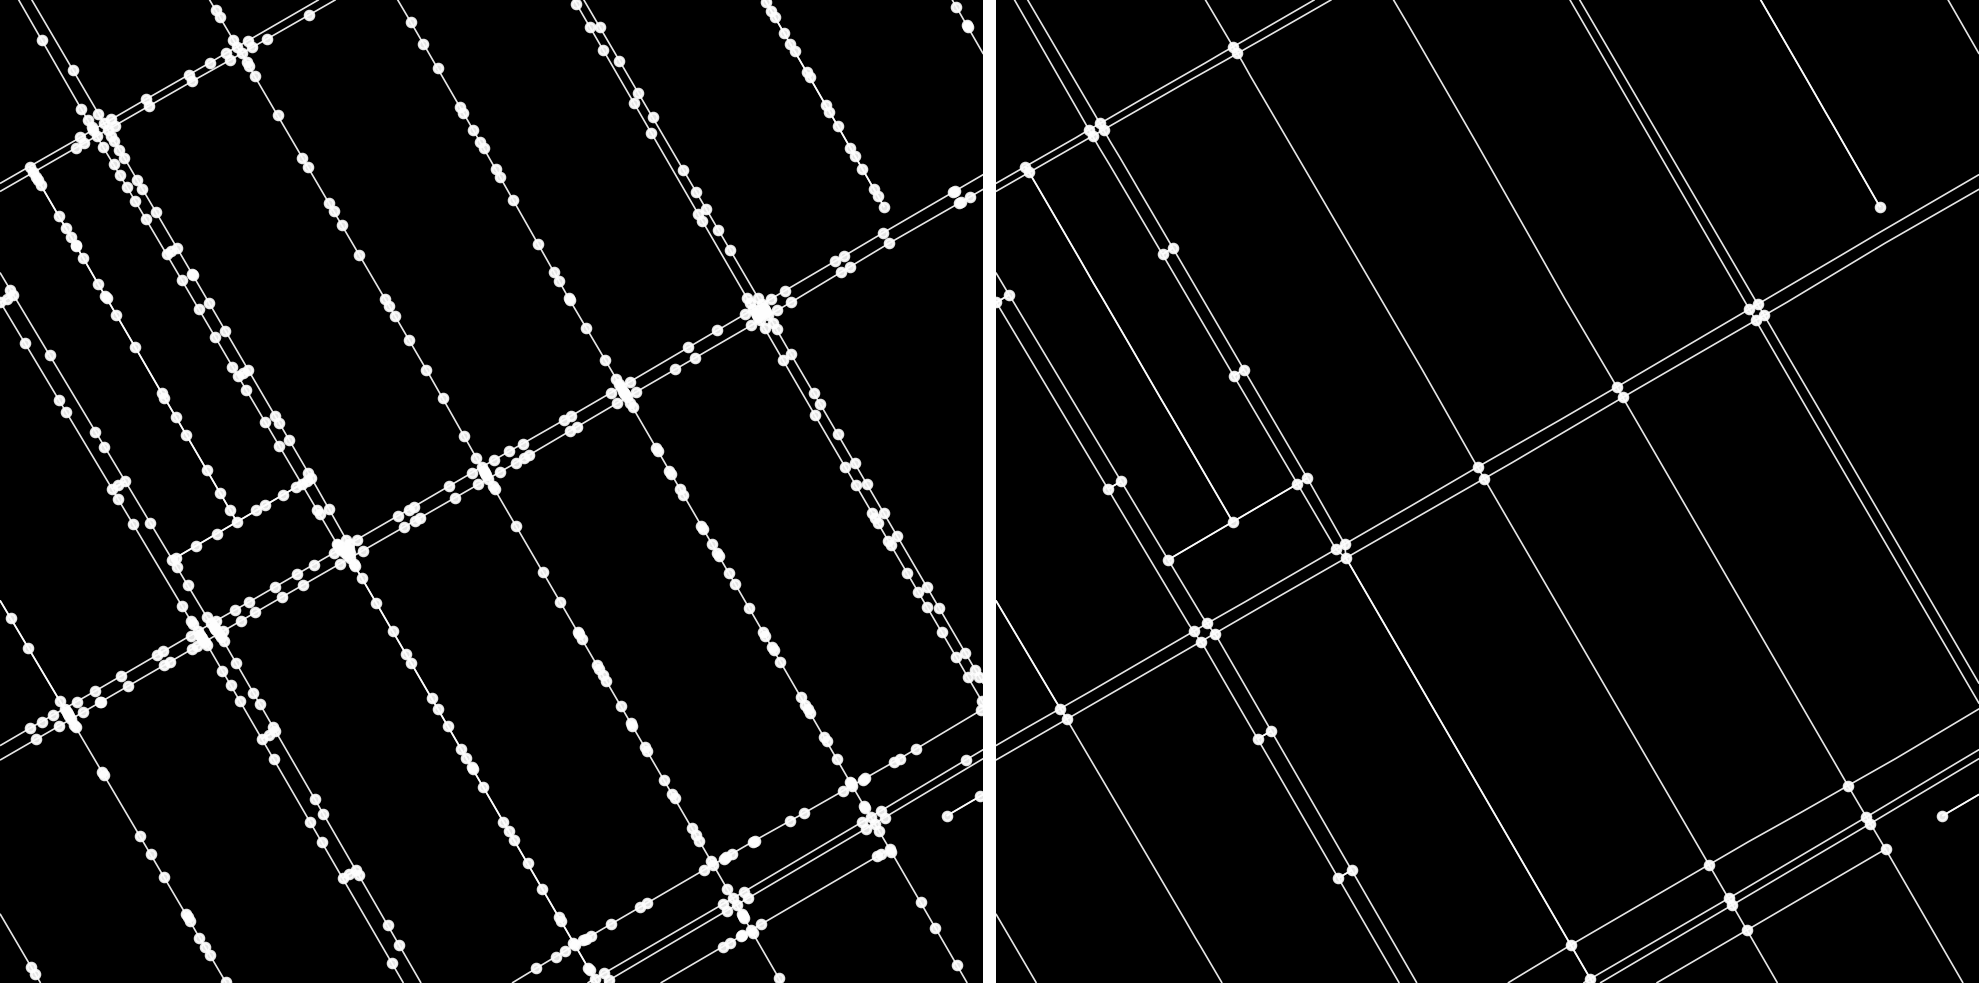
\includegraphics[width=\linewidth]{figures/simplify_comparison}
        \caption{Пример уличной сети до (слева) и после (справа) упрощения рёбер. Упрощение устраняет промежуточные вершины, не соответствующие функциональным узлам сети.}
        \label{fig:simplify_comparison}
        \Description{Пример упрощения графа}
    \end{figure}

    После формирования и упрощения линейного представления сети осуществляется построение графовой структуры.
    Для автомобильной сети учитывается направленность движения: рёбра, не помеченные как односторонние, дублируются с обратным направлением.
    Скорости движения по рёбрам определяются либо напрямую из атрибутов \texttt{maxspeed}, либо, при их отсутствии, на основе типа дороги.
    Время перемещения по ребру вычисляется на основе длины сегмента и назначенной скорости.

    Финальным результатом этапа является ориентированный взвешенный мультиграф \texttt{UrbanGraph} (разд.~\ref{subsec:urban_graph}),
    в котором вершины соответствуют начальным и конечным точкам линейных сегментов, а рёбра — элементам уличной сети с заданной геометрией и весами.
    Таблицы вершин и рёбер формируются векторизованно из массивов координат, без создания промежуточных объектных структур.
    Для пешеходного графа аналогичная процедура применяется с тем отличием, что все рёбра считаются двунаправленными.

    \subsection{Public Transport and Multimodal Graph Construction}
    \label{subsec:public-transport-and-multimodal-graph-construction}

    Для заданной территории и набора поддерживаемых видов транспорта IduEdu извлекает из OpenStreetMap соответствующие объекты \texttt{relation},
    а также связанные с ними элементы уличной сети и остановочной инфраструктуры.
    В случае метрополитена дополнительно запрашиваются станции, платформы и группы пересадок (например, \texttt{stop\_area} и \texttt{stop\_area\_group}),
    что позволяет учитывать подземные переходы и входы/выходы.

    Каждый маршрут общественного транспорта, представленный в OSM в виде отношения, преобразуется в графовую структуру.
    В рамках этого преобразования из relation выделяются элементы, определяющие геометрию движения транспорта по уличной сети,
    а также точки остановок и платформ, соответствующие местам посадки и ожидания пассажиров.
    При этом учитывается, что данные OSM по общественному транспорту не проходят строгую валидацию:
    маршруты могут быть представлены фрагментарно, геометрия пути — разорванной, а остановки или платформы — частично отсутствовать.
    IduEdu обрабатывает такие данные, обеспечивая восстановление непрерывного пути следования маршрута и пары остановка–платформа для каждого участка маршрута.

    На основе непрерывной геометрии формируется ориентированный граф, в котором вершины соответствуют остановкам и платформам,
    а рёбра — сегментам движения транспорта между последовательными остановками (пример на левом фрагменте рис.~\ref{fig:pt_multimodal_example}).
    Дополнительно вводятся пересадочные рёбра, соединяющие остановки с соответствующими платформами.
    Вес таких рёбер настраивается и по умолчанию составляет 1~минуту, моделируя посадку и ожидание транспорта.
    Веса рёбер движения интерпретируются как время перемещения между остановками и вычисляются на основе длины
    геометрического сегмента и эффективной скорости движения, зависящей от настраиваемых характеристик соответствующего вида транспорта и ограничений уличной сети.

    \begin{figure}[htb]
        \centering
        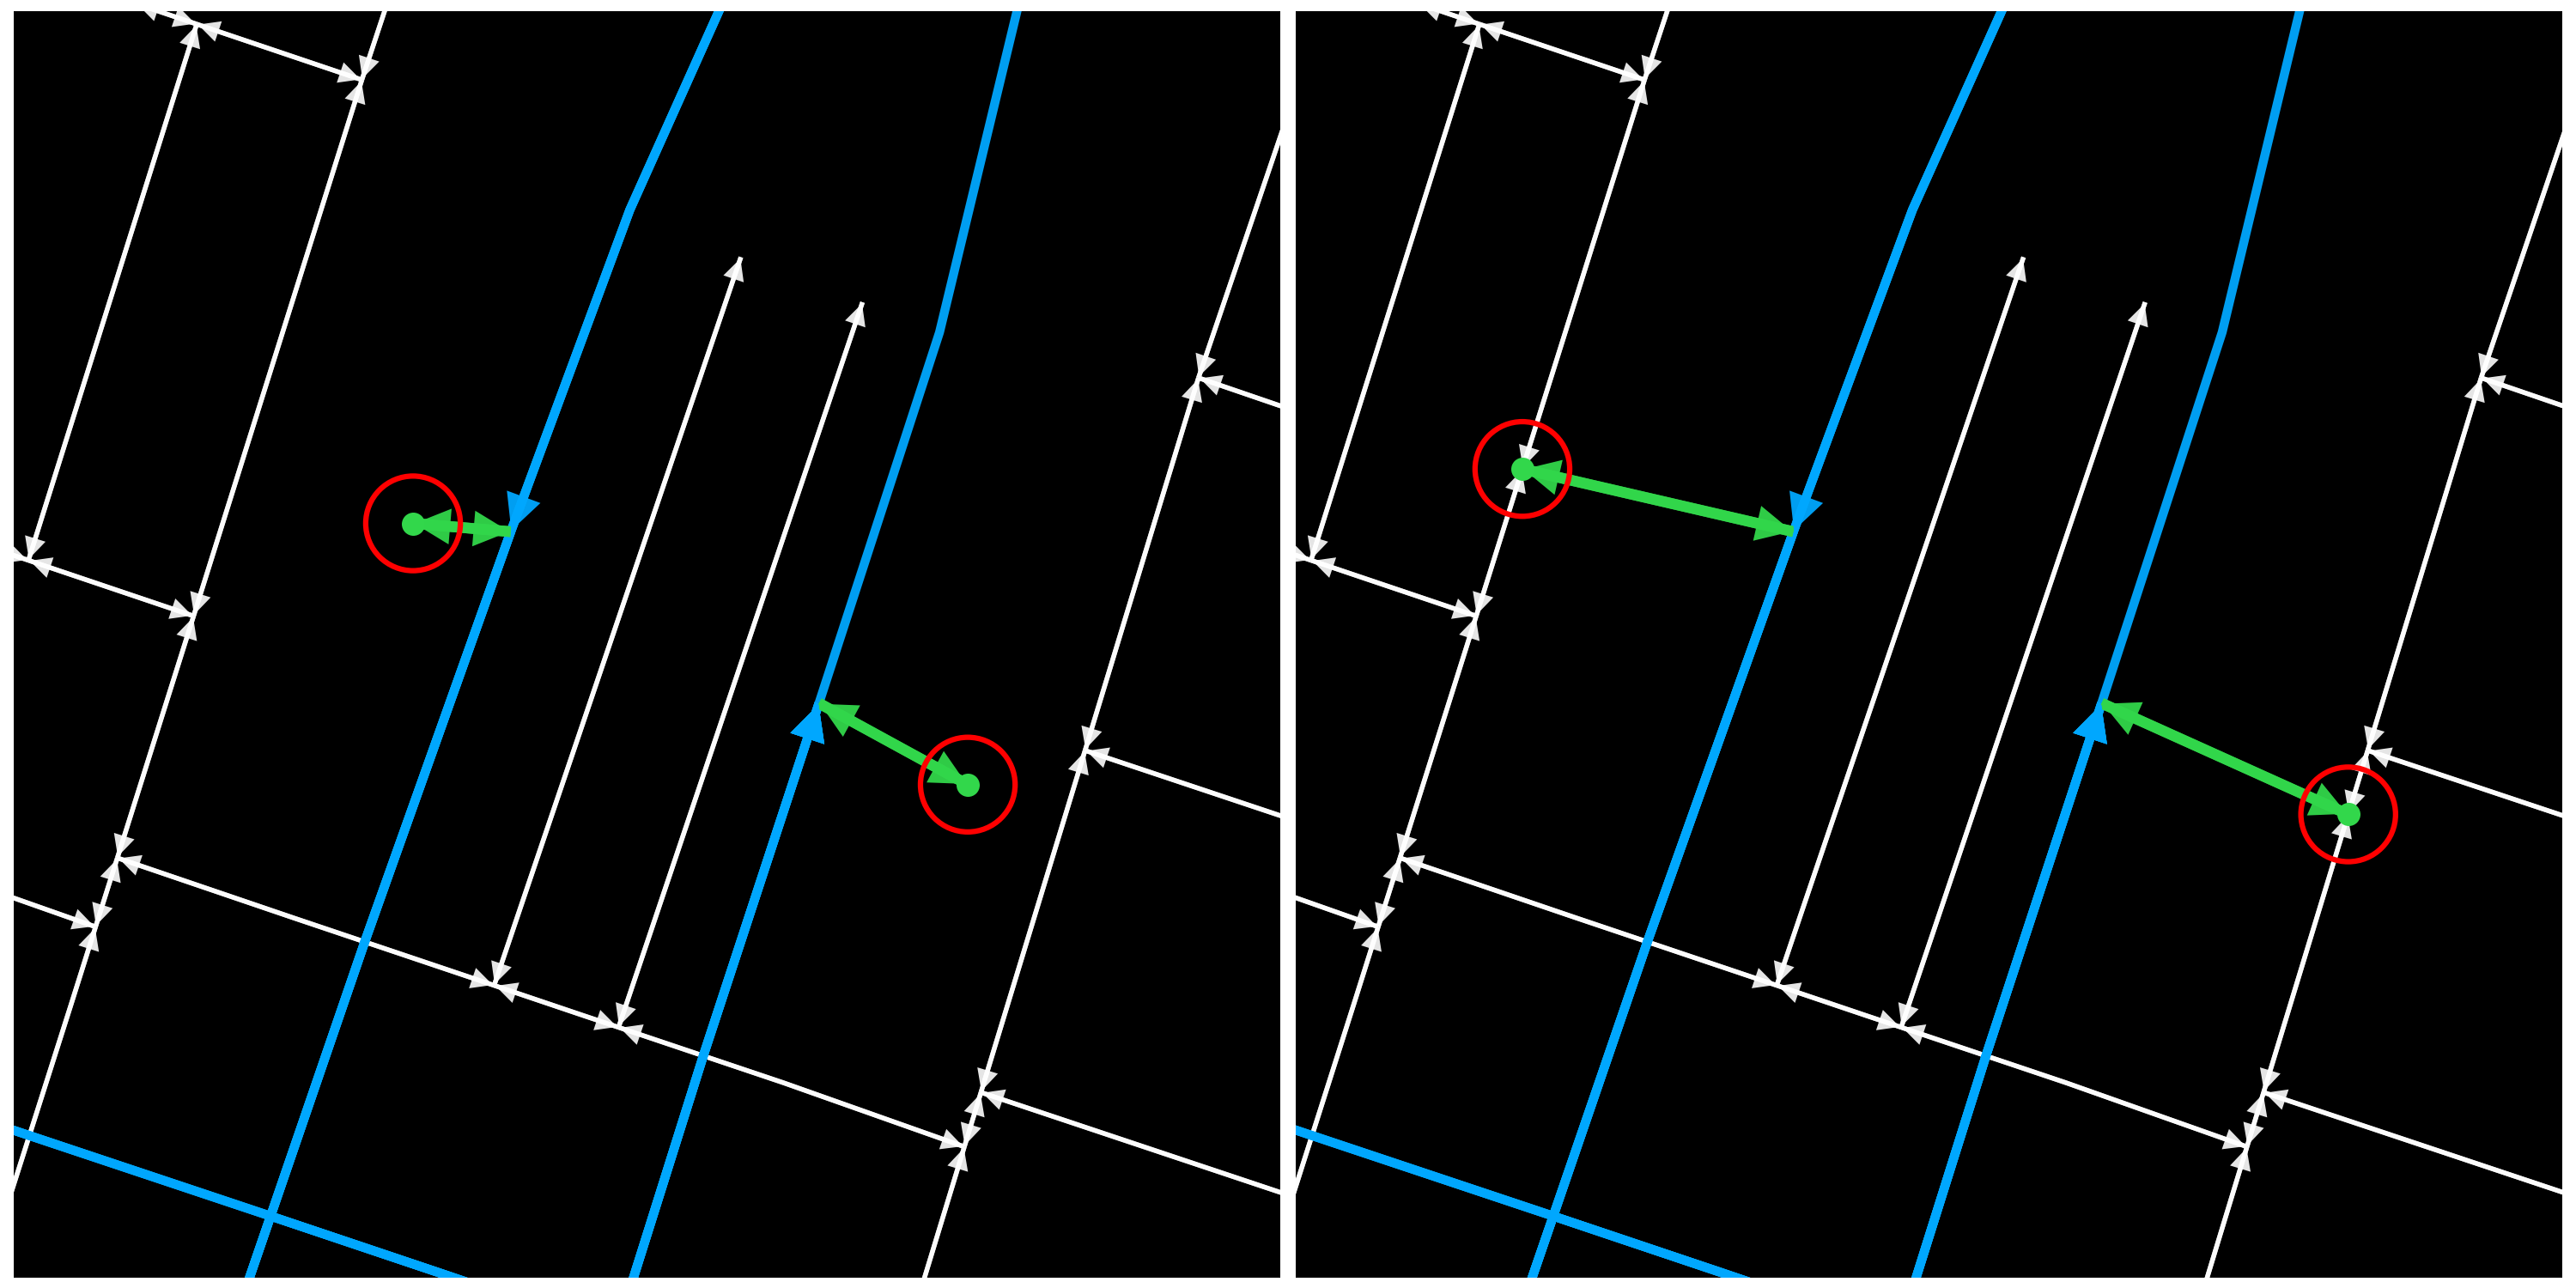
\includegraphics[width=\linewidth]{figures/pt_multimodal_example}
        \caption{Пример построения мультимодального графа. Слева показаны пешеходный граф и граф автобусных маршрутов,
            представленные как отдельные сети. Справа представлен результирующий мультимодальный граф, в котором платформы
            и остановки общественного транспорта спроецированы на рёбра пешеходной сети.}
        \label{fig:pt_multimodal_example}
        \Description{Comparison of separate pedestrian and bus transport graphs (left) and the resulting multimodal graph (right),
            where transit stops are projected onto the pedestrian network to enable integrated multimodal routing.}
    \end{figure}


    Для метрополитена граф расширяется за счёт связей между входами и выходами станций, платформами и точками посадки.
    Если в данных OSM указана глубина станции, то время перемещения по рёбрам входа и выхода моделируется с учётом
    вертикального перемещения (эскалаторы или лифты), что позволяет приблизительно учитывать влияние глубины станции на общее время доступа.
    Несмотря на ограничения существующей структуры данных OSM для подземной инфраструктуры, такой подход обеспечивает
    практичную эвристику моделирования перемещения внутри станций метро.

    После обработки всех маршрутов отдельные графы объединяются в единый граф общественного транспорта.
    Платформы, используемые несколькими маршрутами или видами транспорта, объединяются в общие вершины, обеспечивая корректное моделирование пересадок.
    В результате формируется статический ориентированный \texttt{UrbanGraph} транспортной сети, в котором геометрия рёбер
    отражает фактическое следование транспорта по уличной сети.

    Эти же платформы и входы/выходы станций используются для интеграции транспортного графа с пешеходной сетью при формировании мультимодального графа.
    Для каждой платформы или точки доступа к метро находится ближайшее ребро пешеходного графа в заданном радиусе.
    Точка проецируется на геометрию ребра, которое в результате делится на два сегмента.
    Такая операция не изменяет суммарные веса пешеходных рёбер и сохраняет корректность расстояний, обеспечивая
    при этом связь между пешеходным и транспортным подграфами (правый фрагмент рис.~\ref{fig:pt_multimodal_example}).

    \subsection{OD Matrix Computation with Cutoff}
    \label{subsec:od-matrix-computation-with-cutoff}

    IduEdu поддерживает вычисление матриц корреспонденций (origin--destination, OD) для любого построенного графа
    (пешеходного, автомобильного или мультимодального) между двумя наборами пространственных объектов, заданных в виде \texttt{geopandas.GeoDataFrame}.
    Для согласования геометрии объектов с топологией графа каждая геометрия из наборов источников и назначений
    сопоставляется с ближайшей вершиной графа, что определяет соответствующие точки origin и destination.

    Перед формированием разреженного представления учитывается соотношение мощностей множеств источников и назначений.
    Поскольку алгоритм Дейкстры при запуске из одной вершины вычисляет кратчайшие пути до всех достижимых вершин в пределах фронта поиска,
    вычисление OD-матрицы между $n$ источниками и $m$ целевыми вершинами требует $\min(n, m)$ запусков алгоритма.
    В случае, когда количество источников существенно превышает количество назначений, граф разворачивается путём
    транспонирования его разреженного представления, а роли источников и назначений меняются местами.
    Такой приём позволяет существенно снизить вычислительные затраты без изменения результирующей OD-матрицы.

    Расчёт выполняется по CSR-матрице смежности графа, которая строится непосредственно из таблицы рёбер и кэшируется
    в объекте \texttt{UrbanGraph} (разд.~\ref{subsec:urban_graph}), массив весов (\texttt{float32}) передаётся в JIT-компилируемое
    вычислительное ядро без этапа конвертации графа в вычислительный формат.

    Вычисление OD-матрицы выполняется Numba-ускоренным~\cite{lam2015numba} bounded multi-source вариантом алгоритма Дейкстры,
    реализованным для CSR-представления и распараллеленным по множеству источников.
    Отличием от классической постановки является введение отсечки (cutoff) по весу пути: расширение фронта поиска прекращается при превышении заданного порога,
    что позволяет существенно снизить вычислительные затраты по сравнению с расчётом полной матрицы ``все пары''.
    Поскольку вычислительное представление совпадает с представлением хранения (разд.~\ref{subsec:urban_graph}),
    OD-матрица вычисляется напрямую для графа, сформированного на предыдущих этапах pipeline.

    \subsection{Pipeline Summary}
    \label{subsec:pipeline-summary}

    Предложенный метод реализует целостный и воспроизводимый pipeline анализа городской мобильности,
    охватывающий следующие этапы: извлечение пространственных данных из OpenStreetMap, построение и упрощение уличных графов,
    формирование статического графа общественного транспорта, интеграцию пешеходных и транзитных сетей в единый мультимодальный граф,
    а также масштабируемый расчёт матриц корреспонденций с заданным порогом доступности.
    Все перечисленные этапы выполняются над единым табличным представлением графа в рамках одного инструмента, без смены формата между ними.


    \section{Experimental Evaluation}
    \label{sec:experiments}

    Все эксперименты выполнялись на рабочей станции с процессором Intel Core i7-12700F и 64~GB оперативной памяти (Windows, Python~3.11.9).
    Ключевые версии библиотек: IduEdu~2.0.0, OSMnx~2.1.0, Pyrosm~0.11.0, NetworkX~3.6.1, NetworKit~11.2.1, igraph~1.0.0, Numba~0.65.1, GeoPandas~1.1.4, Shapely~2.1.2, SciPy~1.17.1;
    полный список версий для каждого прогона фиксируется в файлах \texttt{env\_*.json} репозитория.
    Полный код бенчмарков (resume-safe, с фиксированными seed'ами), сырые CSV-результаты и ноутбуки для воспроизведения
    всех графиков опубликованы в репозитории проекта\footnote{Ссылка на репозиторий и архивную версию (DOI) будет указана в camera-ready.}.
    Каждое измерение повторялось не менее трёх раз; в анализе используются медианные значения, а разброс между повторами
    приводится в сопровождающих ноутбуках.
    Перед измерениями выполнялся прогрев (заполнение кешей Overpass-запросов, JIT-компиляция Numba-ядер, первичный импорт библиотек), не учитываемый в результатах.

    \subsection{Street Graph Construction Benchmarks}
    \label{subsec:build_benchmark}

    В эксперименте по сборке уличных графов (B1) сравнивается производительность и результирующие характеристики построения пешеходных
    и автомобильных графов для трёх Python-инструментов: \textbf{OSMnx}, \textbf{Pyrosm} и \textbf{IduEdu}.
    Пешеходная сеть является наиболее показательным случаем за счёт большего числа вершин и рёбер из-за высокой детализации уличной инфраструктуры;
    автомобильная сеть добавляет обработку направленности движения.

    Для обеспечения корректности сравнения все инструменты использовали одну и ту же область интереса (AOI):
    для каждого города загружался PBF-файл OpenStreetMap, из заголовка которого извлекалась охватывающая bounding box;
    она же применялась в качестве геометрического запроса для OSMnx и IduEdu.
    Города подобраны по возрастанию масштаба: Helsinki, Санкт-Петербург, Москва, Лондон, Сеул, Нью-Йорк.
    Для OSMnx и IduEdu дополнительно сравнивались режимы с включённым и отключённым упрощением графа (\texttt{simplify=True/False});
    Pyrosm сопоставимого переключателя не имеет.

    В сопоставимом режиме с включённым упрощением IduEdu устойчиво опережает OSMnx при построении пешеходных графов:
    медианное ускорение по шести городам составляет около $5.7\times$ (от $3.3\times$ на Нью-Йорке до $6.0\times$ на Хельсинки),
    а без упрощения достигает $\approx 9\times$.
    В абсолютных значениях пешеходный граф Санкт-Петербурга собирается за ${\approx}20$~с против ${\approx}115$~с у OSMnx и ${\approx}95$~с у Pyrosm.
    Для автомобильной сети, где дополнительно обрабатывается направленность движения, ускорение относительно OSMnx составляет $\approx 4$--$5\times$.
    Сводные результаты представлены на рис.~\ref{fig:walk_graph_benchmark}.

    \begin{figure}[htb]
        \centering
        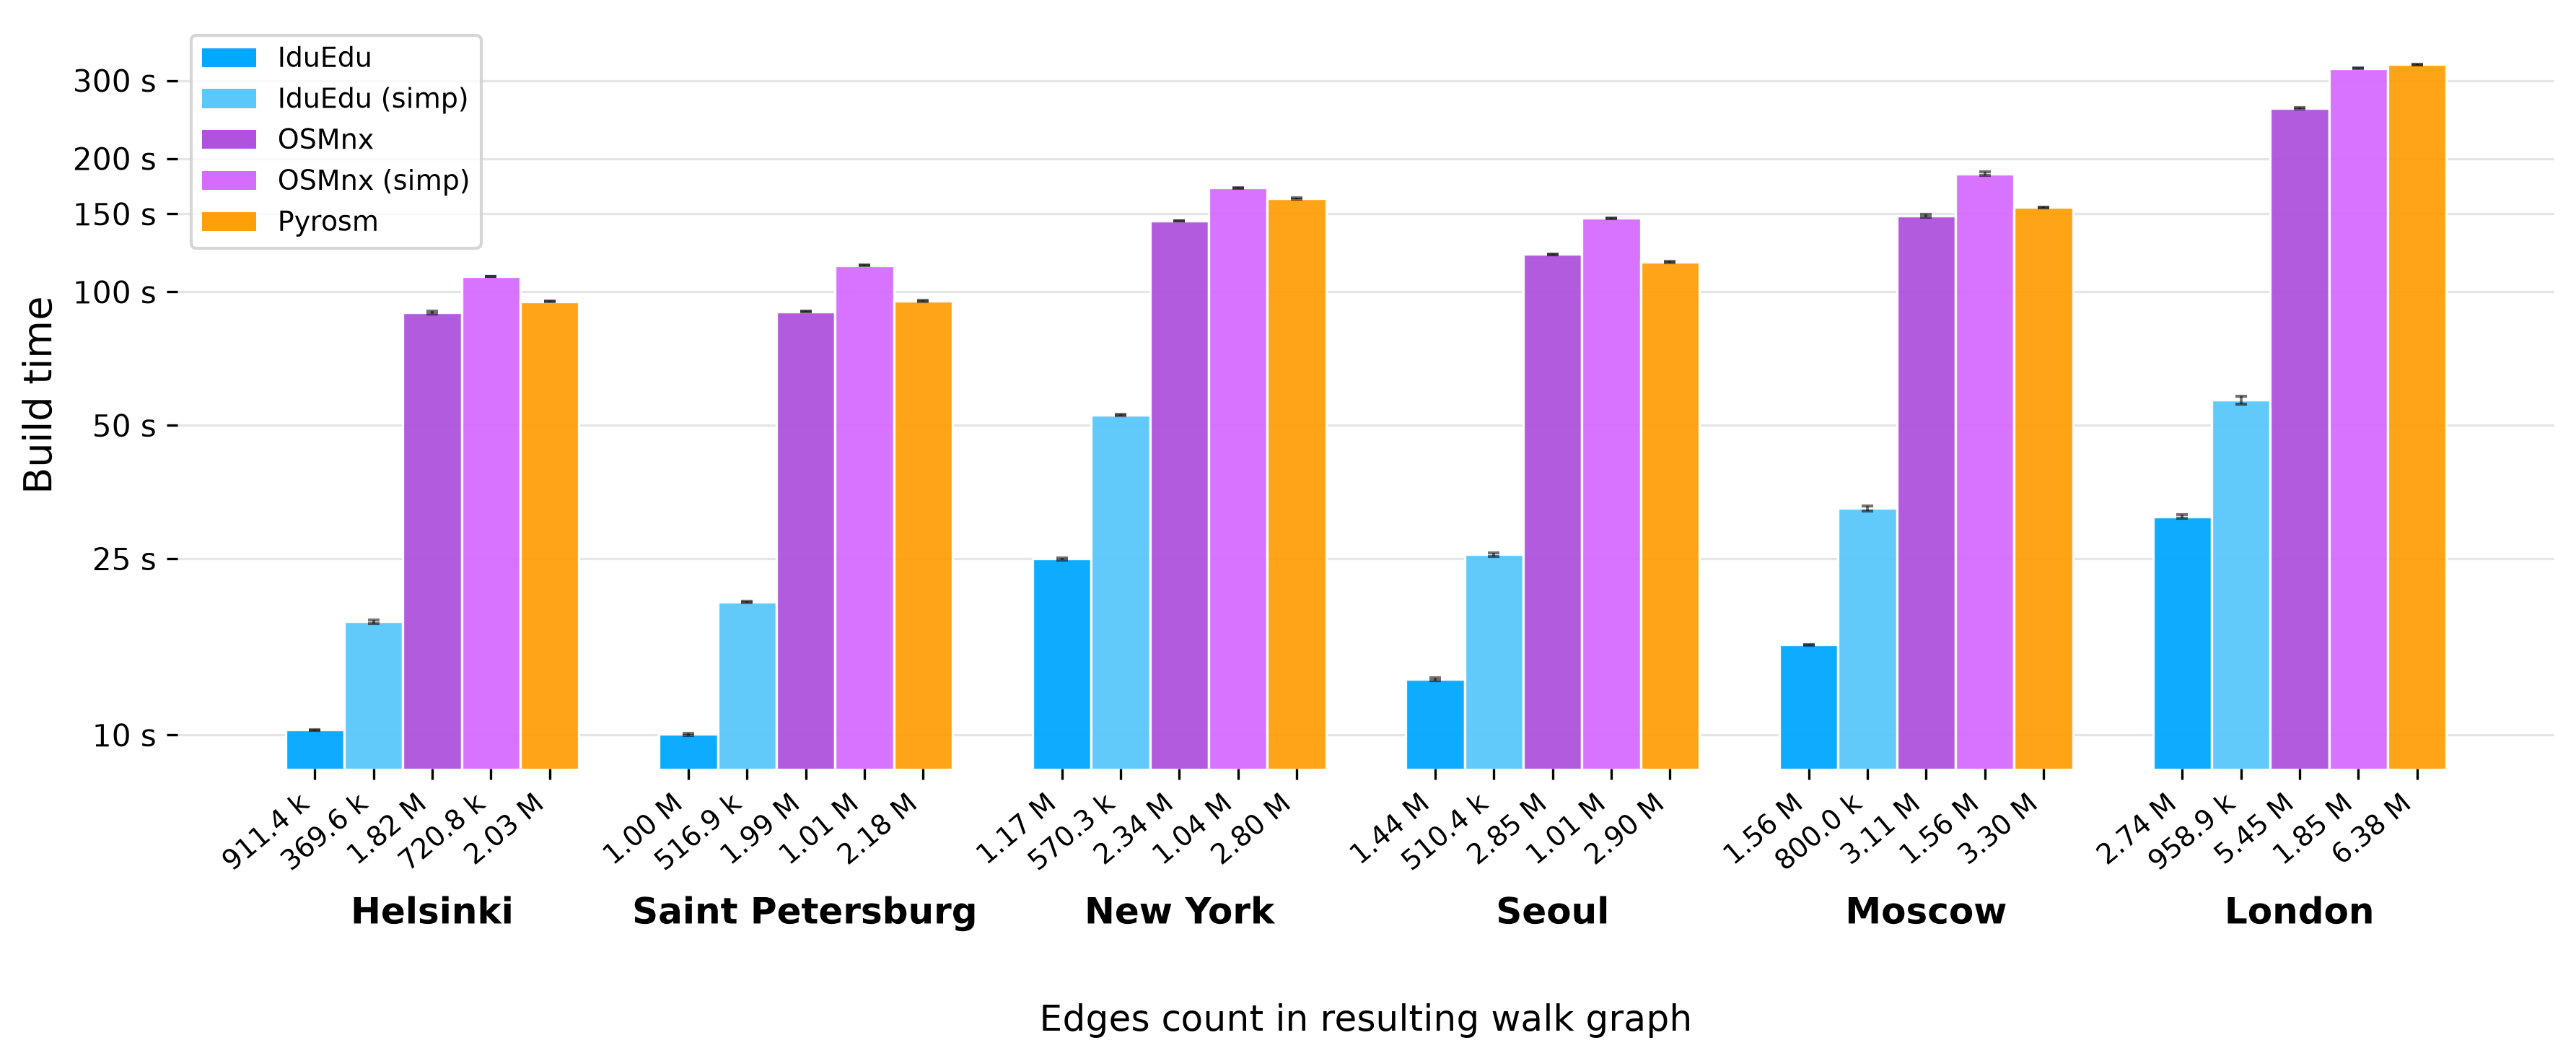
\includegraphics[width=\linewidth]{figures/build_benchmark_walk}
        \caption{Сравнение производительности построения пешеходных графов для OSMnx, Pyrosm и IduEdu.
        Показаны время построения и количество рёбер для различных городов, а также влияние включения и отключения упрощения графа.}
        \label{fig:walk_graph_benchmark}
        \Description{Benchmark results comparing pedestrian graph construction time and graph size across different libraries and simplification settings.}
    \end{figure}

    \subsection{Multimodal Graph Construction Benchmarks}
    \label{subsec:multimodal-graph-construction-benchmarks}

    В эксперименте по мультимодальной сборке (B2) оценивается время построения мультимодального графа в IduEdu для выбранных городов.
    Границы областей интереса совпадают с областями, использованными в предыдущем эксперименте.
    Для каждой территории последовательно выполнялось построение пешеходного графа, графа общественного транспорта
    (автобусы, трамваи, троллейбусы и метрополитен), а затем их интеграция в единый мультимодальный граф.

    Для каждого города измерялось время выполнения и количество рёбер на каждом этапе pipeline: построение пешеходной сети,
    построение транспортного графа и операция объединения (join).
    Полный цикл построения мультимодального графа выполнялся три раза, после чего в анализ включались медианные значения.
    Сводные результаты эксперимента представлены на рис.~\ref{fig:intermodal_benchmark} и иллюстрируют вклад отдельных
    этапов в общее время построения мультимодального графа для городов различного масштаба и структуры транспортной сети.

    \begin{figure}[tbh]
        \centering
        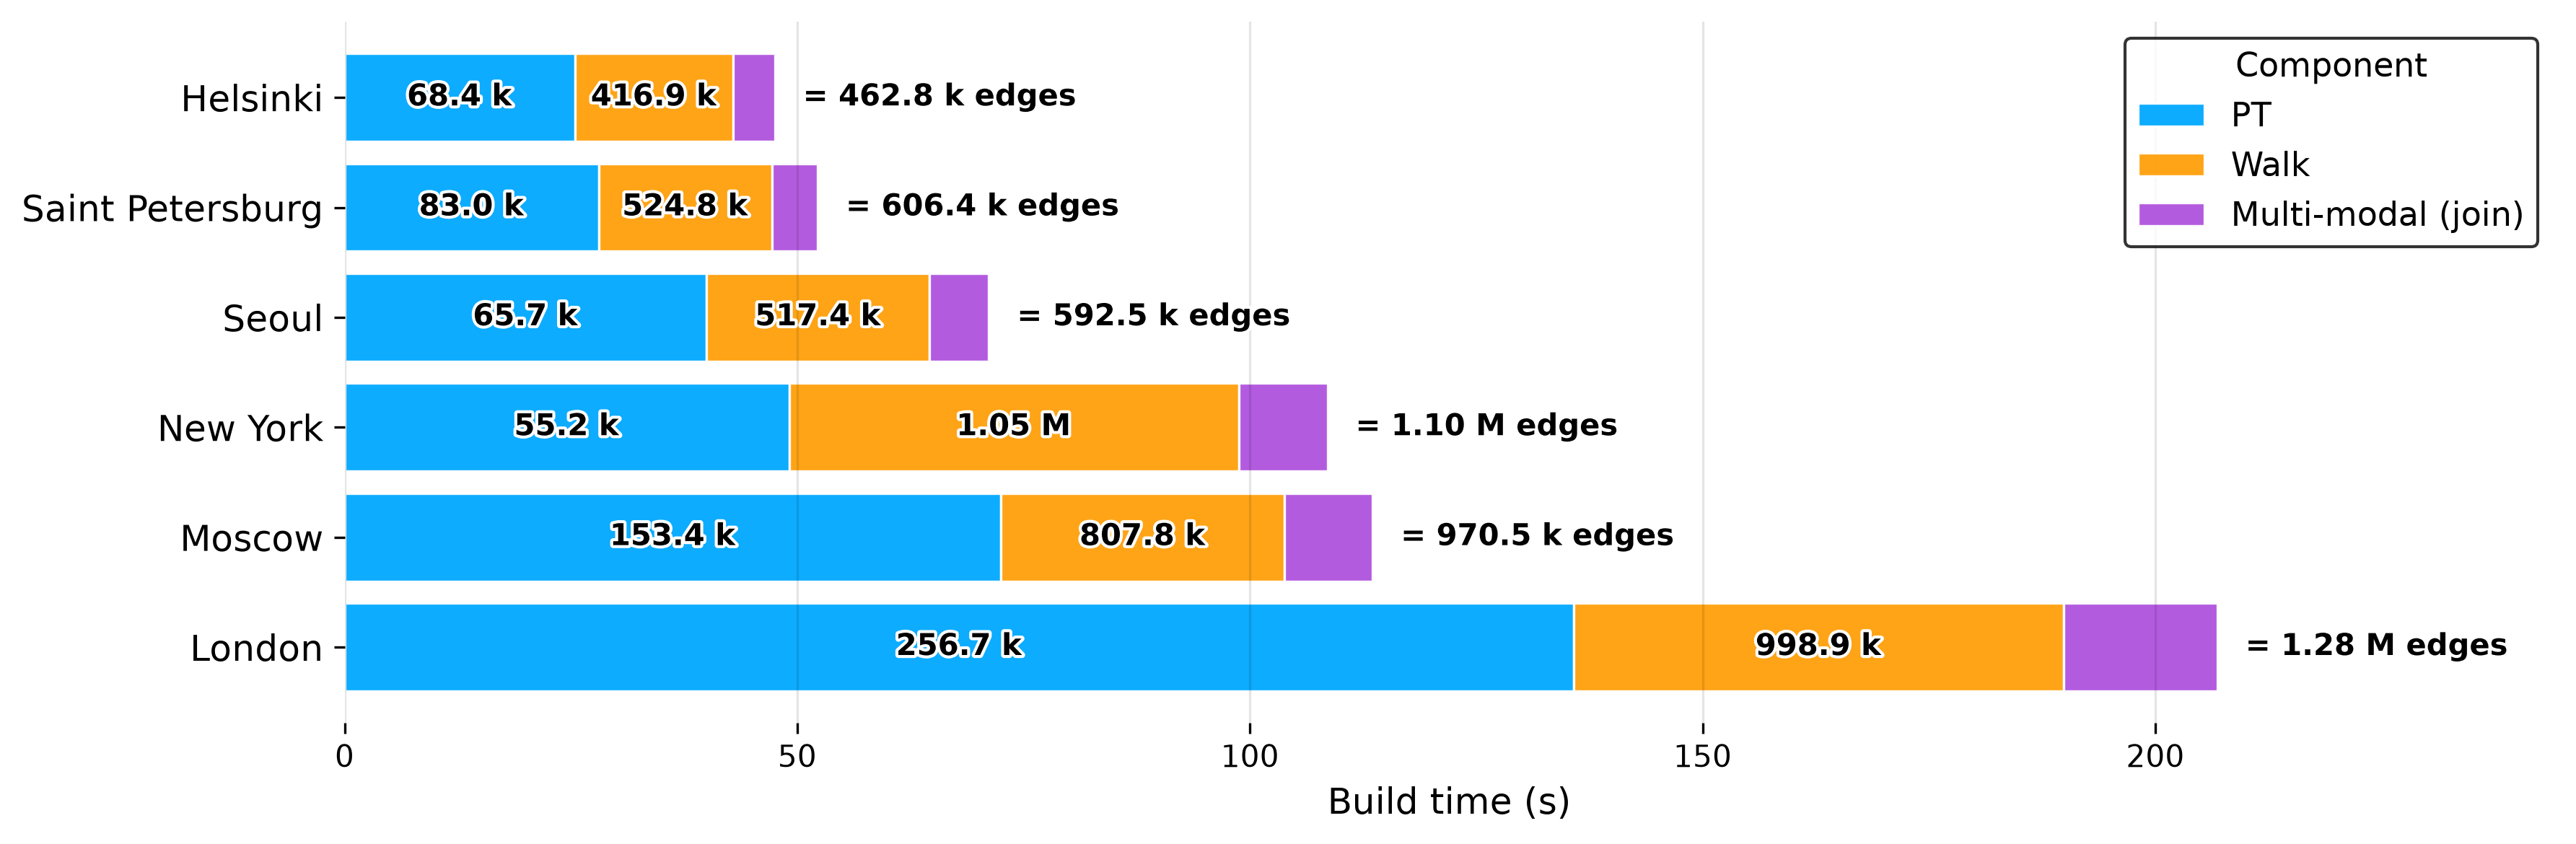
\includegraphics[width=\linewidth]{figures/intermodal_stacked_time_by_city}
        \caption{Время построения мультимодального графа в IduEdu для различных городов с разложением по этапам pipeline:
        построение графа общественного транспорта (PT), построение пешеходного графа (Walk) и их интеграция в единый
        мультимодальный граф (Join). Подписи внутри столбцов отражают количество рёбер на соответствующем этапе.}
        \label{fig:intermodal_benchmark}
        \Description{Stacked bar chart showing multimodal graph construction time across cities, decomposed into public
        transport graph construction, pedestrian graph construction, and their integration.}
    \end{figure}

    \subsection{Memory Footprint}
    \label{subsec:memory_benchmark}

    Табличное представление графа влияет не только на скорость, но и на размер итогового объекта в памяти.
    Поэтому в эксперименте по сборке графов (B1) дополнительно измеряется \emph{in-memory graph representation size}: детерминированный размер уже построенного представления графа.
    Для IduEdu учитывается объект \texttt{UrbanGraph}: таблицы вершин и рёбер \texttt{GeoDataFrame} вместе с буферами координат геометрий Shapely.
    Для OSMnx и Pyrosm измеряется возвращаемый ими \texttt{networkx.MultiDiGraph}, то есть объектное представление пространственного OSM-графа с геометрией и атрибутами.

    Такой протокол сравнивает пространственные представления графа, а не вычислительные контейнеры без геометрии.
    Результаты на рис.~\ref{fig:memory_benchmark}, построенные из тех же прогонов B1, показывают, что колоночное хранение
    \texttt{UrbanGraph} существенно компактнее объектных NetworkX-представлений при сохранении сопоставимой пространственной информации:
    для пешеходного графа Санкт-Петербурга (\texttt{simplify=True}) \texttt{UrbanGraph} занимает ${\approx}76$~МБ против ${\approx}865$~МБ у \texttt{MultiDiGraph} OSMnx (также \texttt{simplify=True})
    и ${\approx}5.7$~ГБ у сырого, не упрощённого графа Pyrosm.

    \begin{figure}[htb]
        \centering
        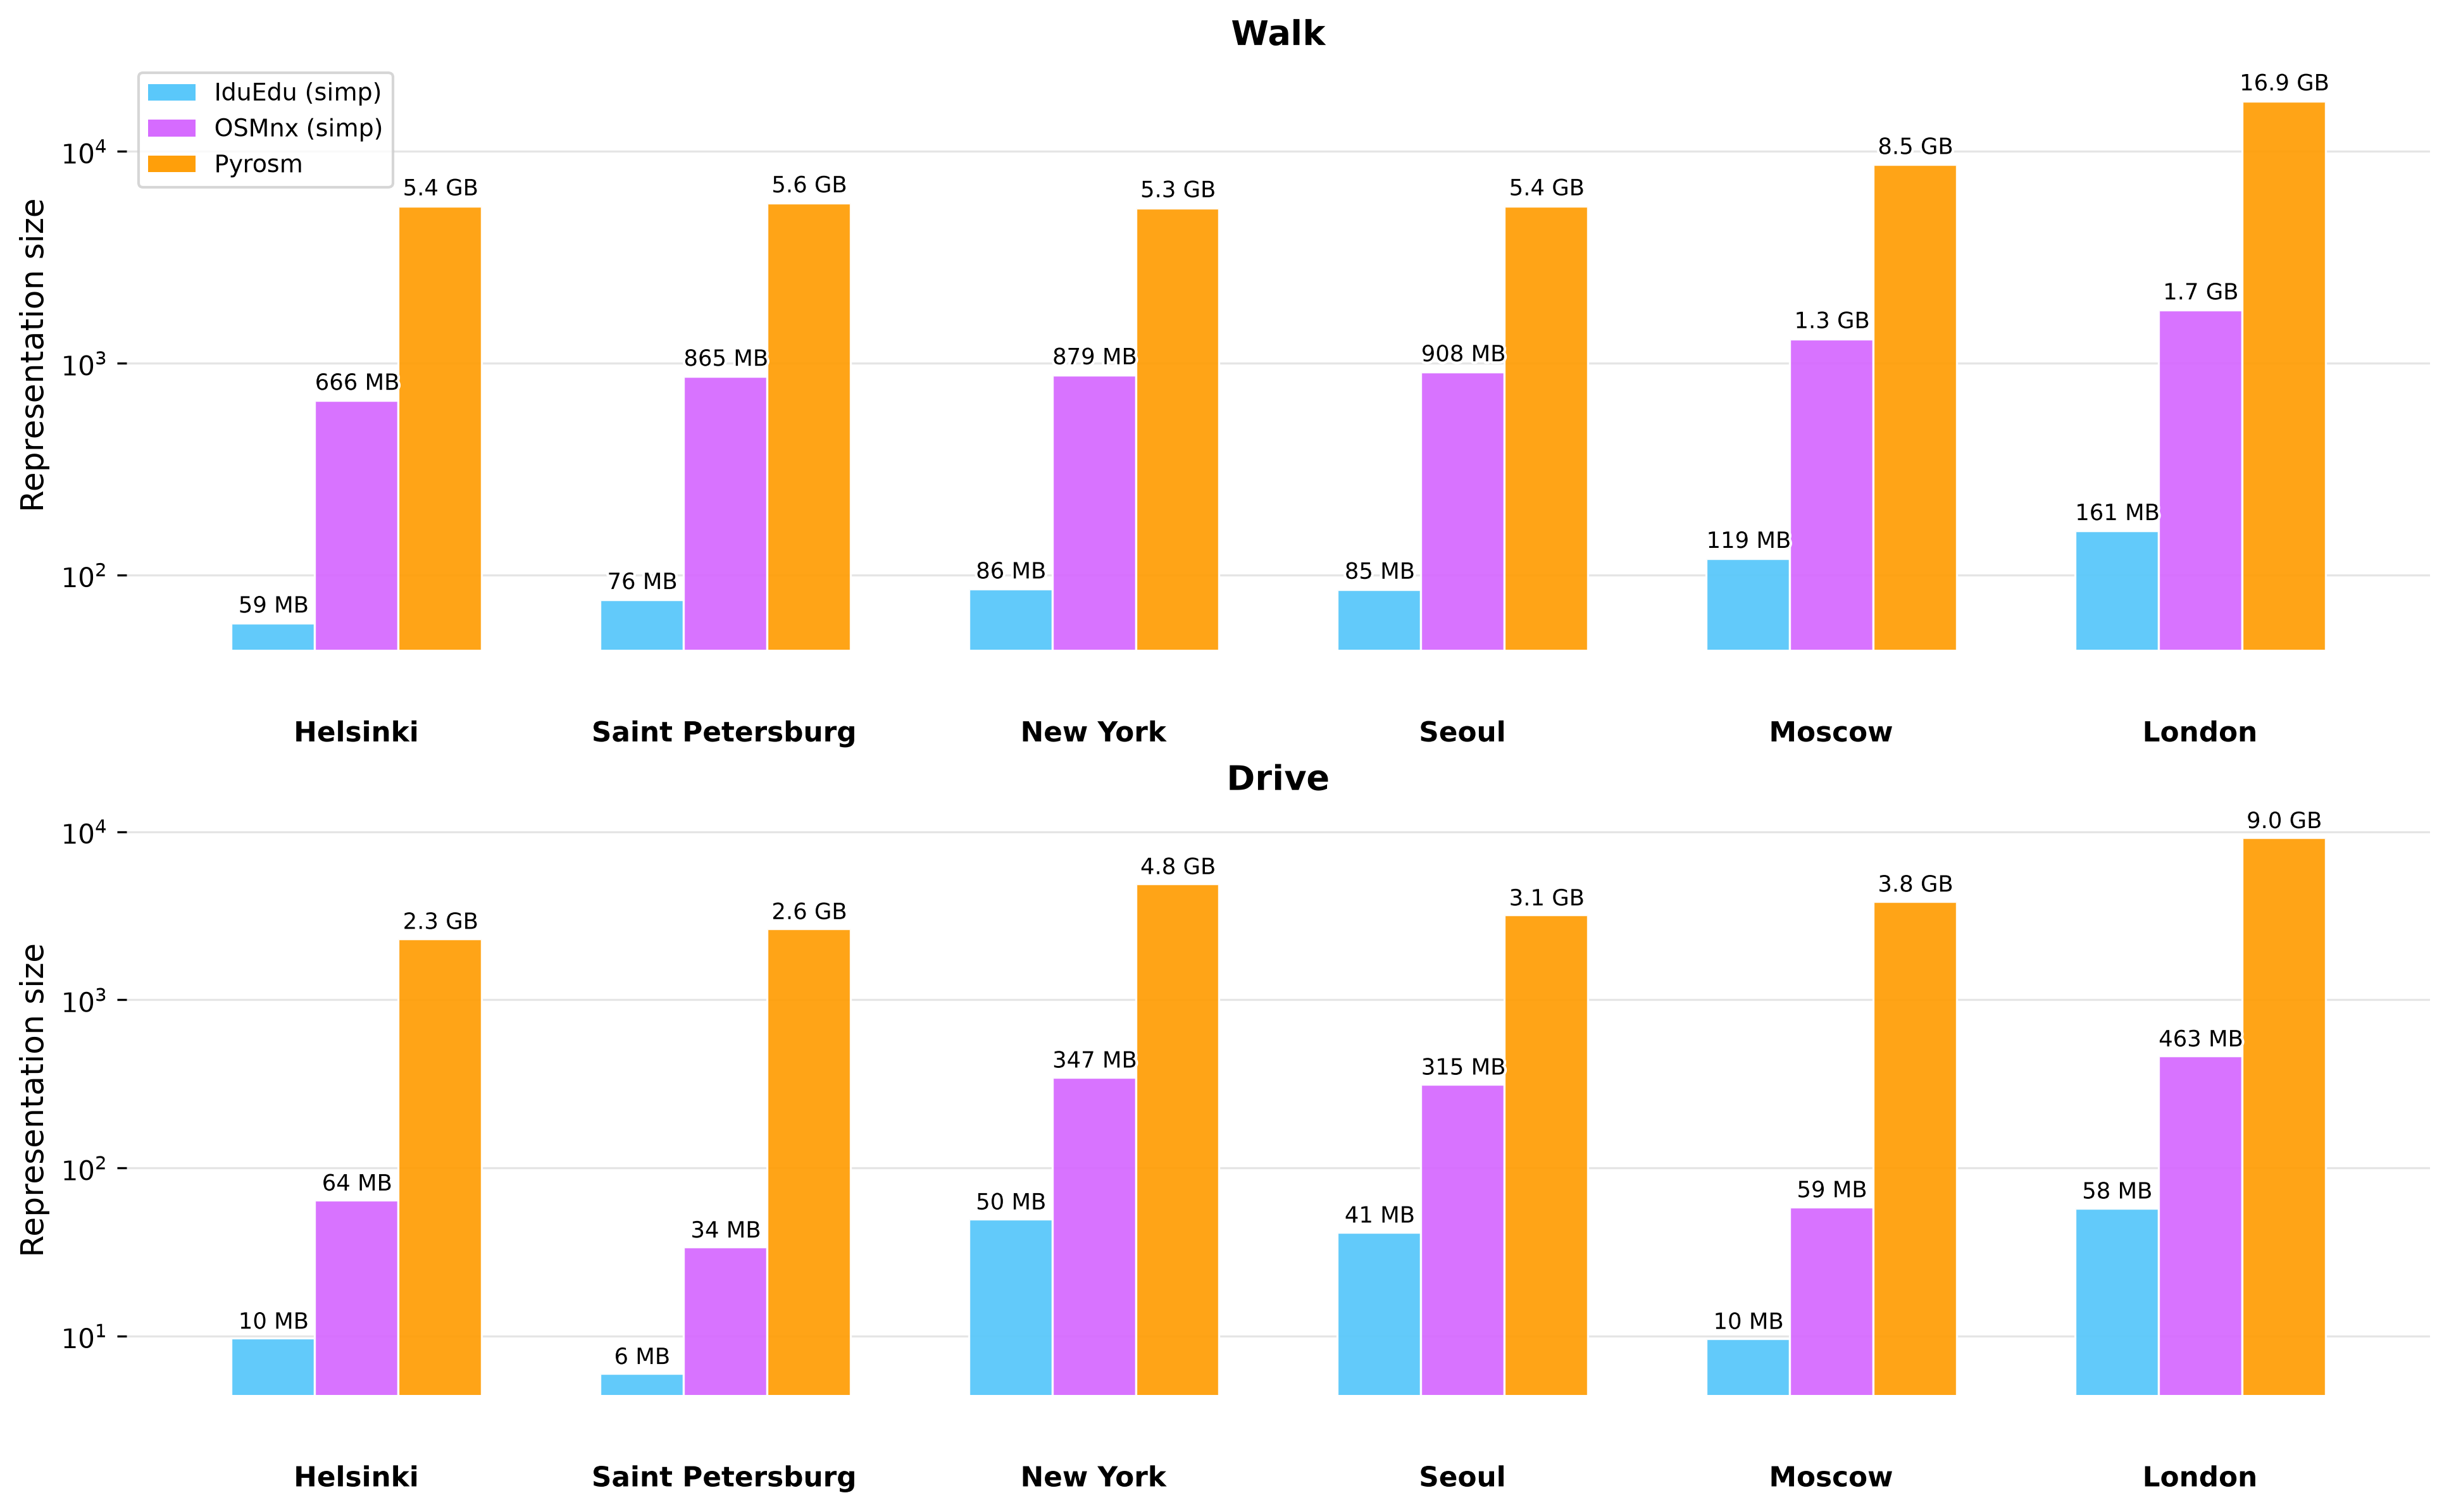
\includegraphics[width=\linewidth]{figures/memory_benchmark}
        \caption{Размер итогового представления графа в памяти для IduEdu, OSMnx и Pyrosm по данным эксперимента B1.}
        \label{fig:memory_benchmark}
        \Description{Bar chart comparing in-memory representation size of graph objects returned by IduEdu, OSMnx, and Pyrosm.}
    \end{figure}

    \subsection{Result Validity}
    \label{subsec:validity}

    Сравнение производительности осмысленно только при совпадении результатов, поэтому отдельно проверяется корректность вычислений.
    Во-первых, OD-матрица IduEdu сопоставляется с эталонным расчётом NetworkX на идентичном графе: множества
    достижимости совпадают полностью, а максимальное расхождение конечных значений не превышает $3\cdot10^{-4}$~минуты и
    объясняется накоплением ошибки округления \texttt{float32}-арифметики вычислительного ядра относительно \texttt{float64}-эталона.
    Во-вторых, сопоставляются пешеходные графы IduEdu и OSMnx, построенные для одной территории: при различающихся
    по построению правилах упрощения суммарная протяжённость сети совпадает с точностью около 1\%, подтверждающая эквивалентность извлечённых сетей.

    \subsection{OD Matrix Computation Benchmarks}
    \label{subsec:od_benchmark}

    В эксперименте по расчёту OD-матриц (B3) сравнивается время вычисления матриц кратчайших путей (origin--destination, OD) для трёх библиотек:
    \textbf{IduEdu}, \textbf{NetworKit} и \textbf{igraph}.
    Во всех экспериментах используется один и тот же мультимодальный граф городской транспортной сети Санкт-Петербурга,
    предварительно построенный в IduEdu и взвешенный по атрибуту времени перемещения.

    Протокол сравнения отражает реальный рабочий процесс каждого инструмента.
    Для обеспечения честности конкурирующие библиотеки стартуют не из внутреннего представления IduEdu,
    а из графа \texttt{networkx.MultiDiGraph} — стандартного представления, которое производит экосистема osmnx/networkx.
    Этот граф строится из того же \texttt{UrbanGraph} (идентичная топология и веса, развёрнутые односторонние рёбра, сохранённые координаты вершин),
    поэтому все инструменты маршрутизируют по одной и той же сети.
    Далее каждый конкурент оплачивает те же издержки, что и на практике: конвертацию \texttt{networkx} в собственный формат библиотеки
    (со схлопыванием параллельных рёбер по минимальному весу) и пространственную привязку объектов к вершинам — построение
    собственного пространственного индекса (\texttt{scipy.cKDTree}) по координатам вершин и запрос ближайших вершин.
    Для конкурентов эти этапы (convert и snap) измеряются отдельно от чистого времени расчёта OD; приводится как чистое, так и суммарное (end-to-end) время.

    В отличие от них, IduEdu принимает собственный \texttt{UrbanGraph} (результат своих же строителей) и выполняет привязку внутренне через персистентный
    R-tree индекс \texttt{GeoDataFrame}, поэтому этап конвертации для него отсутствует по построению, а привязка входит в общее время расчёта.
    Отметим, что сам NetworkX в OD-сравнении не участвует как маршрутизатор (у него нет пакетного OD-API);
    он используется лишь как общее исходное представление, из которого конкуренты выполняют конвертацию.

    Основным межбиблиотечным сравнением является режим полного расчёта (full): IduEdu без отсечки сопоставляется
    с NetworKit и igraph, выполняющими такой же полный расчёт кратчайших путей.
    Дополнительно для IduEdu приводятся кривые с различными значениями порога отсечки; поскольку в NetworKit и igraph
    отсутствует сопоставимый механизм cutoff-поиска, они всегда выполняют полный обход, и cutoff-режим IduEdu
    следует интерпретировать как отдельное прикладное преимущество на задачах локальной доступности.

    Эксперимент проводится в двух постановках, позволяющих отдельно оценить влияние соотношения числа источников и назначений:
    (i) прямоугольные OD-матрицы (origins $\rightarrow$ destinations) и (ii) квадратные OD-матрицы (origins $\rightarrow$ origins).

    В первой постановке множество источников формируется из объектов жилой застройки,
    а множество назначений — из точек социальных объектов (школ), число которых фиксировано и составляет  $|D|=911$.
    Источники выбираются случайно, при этом один и тот же поднабор используется для всех библиотек и всех повторов эксперимента.
    Размер множества источников $|O|$ последовательно увеличивается от $128$ до $131{,}072$ при фиксированном числе назначений.

    Результаты эксперимента для прямоугольных OD-матриц представлены на рис.~\ref{fig:od_time_rect}.
    При увеличении числа источников характер зависимости времени вычислений для IduEdu принципиально отличается от NetworKit и igraph.
    В режиме полного расчёта время выполнения IduEdu слабо растёт и остаётся в пределах десятков секунд (${\approx}50$~с при $|O|=1{,}024$ и ${\approx}80$~с при $|O|=32{,}768$),
    тогда как у NetworKit и igraph наблюдается нелинейный рост.
    Такое различие связано с применением разворота графа при $|O| > |D|$, в результате которого число запусков алгоритма
    кратчайших путей эффективно определяется меньшим множеством стартовых вершин.


    \begin{figure}[htb]
        \centering
        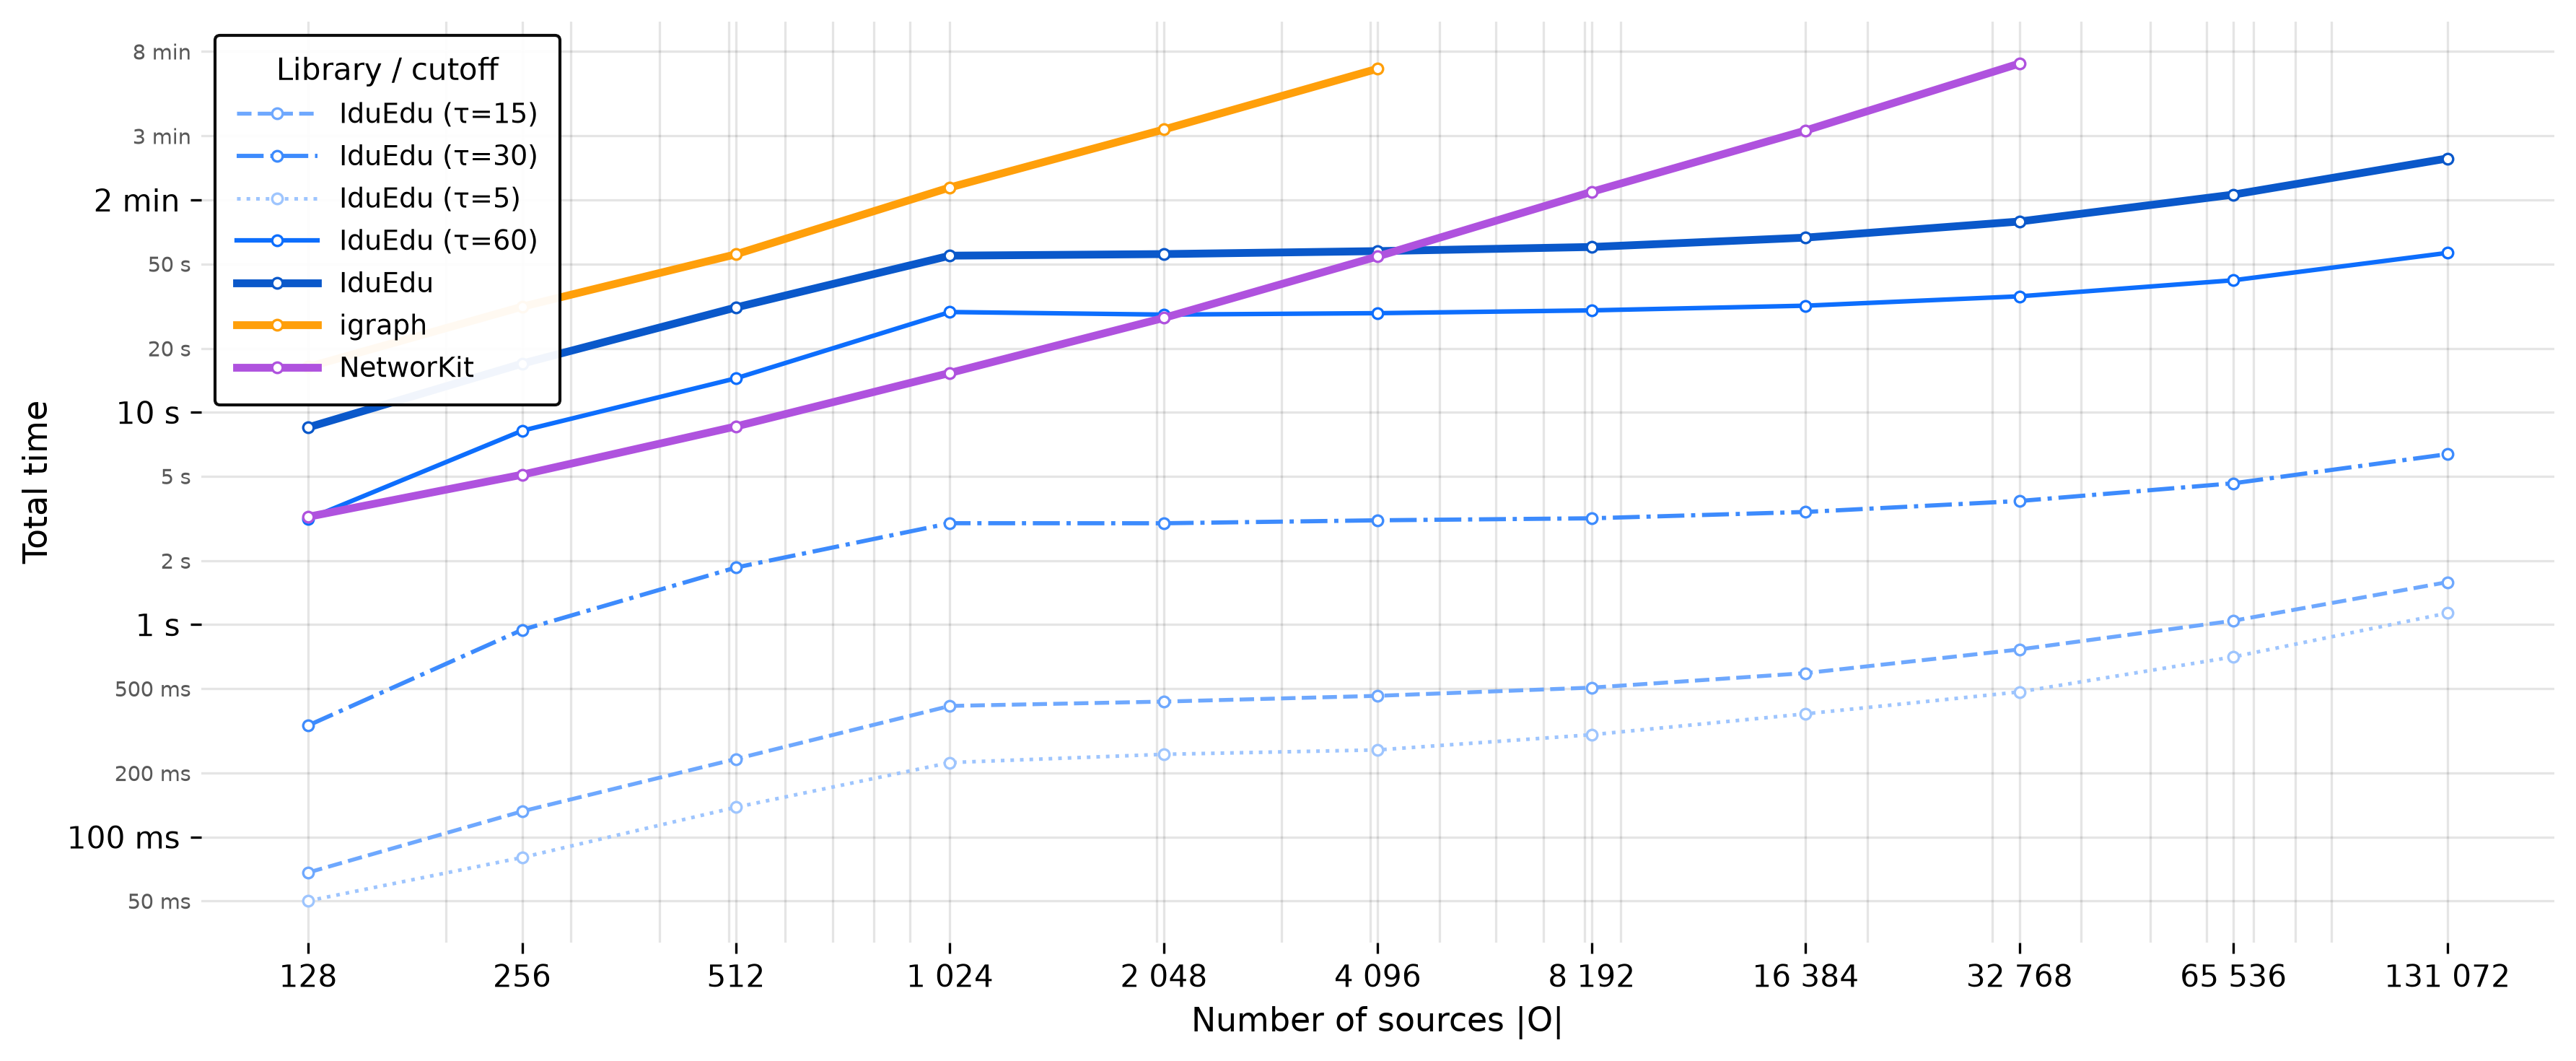
\includegraphics[width=\linewidth]{figures/od_time_rect}
        \caption{Время вычисления прямоугольных OD-матриц (origins $\rightarrow$ destinations)
            для IduEdu, NetworKit и igraph в зависимости от числа источников.
            Для IduEdu показано влияние различных значений порога отсечки по времени пути.}
        \label{fig:od_time_rect}
        \Description{OD matrix computation time for rectangular origin-destination settings,
            comparing IduEdu with different cutoffs against NetworKit and igraph.}
    \end{figure}

    Во второй постановке вычисляются квадратные OD-матрицы, в которых множества источников и назначений совпадают ($|O| = |D|$).
    Для каждого значения размерности выбирается фиксированная случайная подвыборка объектов жилой застройки,
    используемая одновременно как origins и destinations, что приводит к матрицам размера $|O|\times|O|$.

    В этом режиме эффект разворота графа отсутствует, и вычислительная сложность определяется непосредственно числом источников.
    Как показано на рис.~\ref{fig:od_time_square}, в режиме полного расчёта без отсечки IduEdu демонстрирует монотонный
    рост времени выполнения и уступает NetworKit.
    Однако введение временной отсечки приводит к качественному изменению поведения: при порогах 5–30 мин время выполнения
    IduEdu демонстрирует значительно более слабую зависимость от роста $|O|$.
    Такое поведение коррелирует с увеличением доли недостижимых пар и уменьшением глубины обхода графа.


    \begin{figure}[htb]
        \centering
        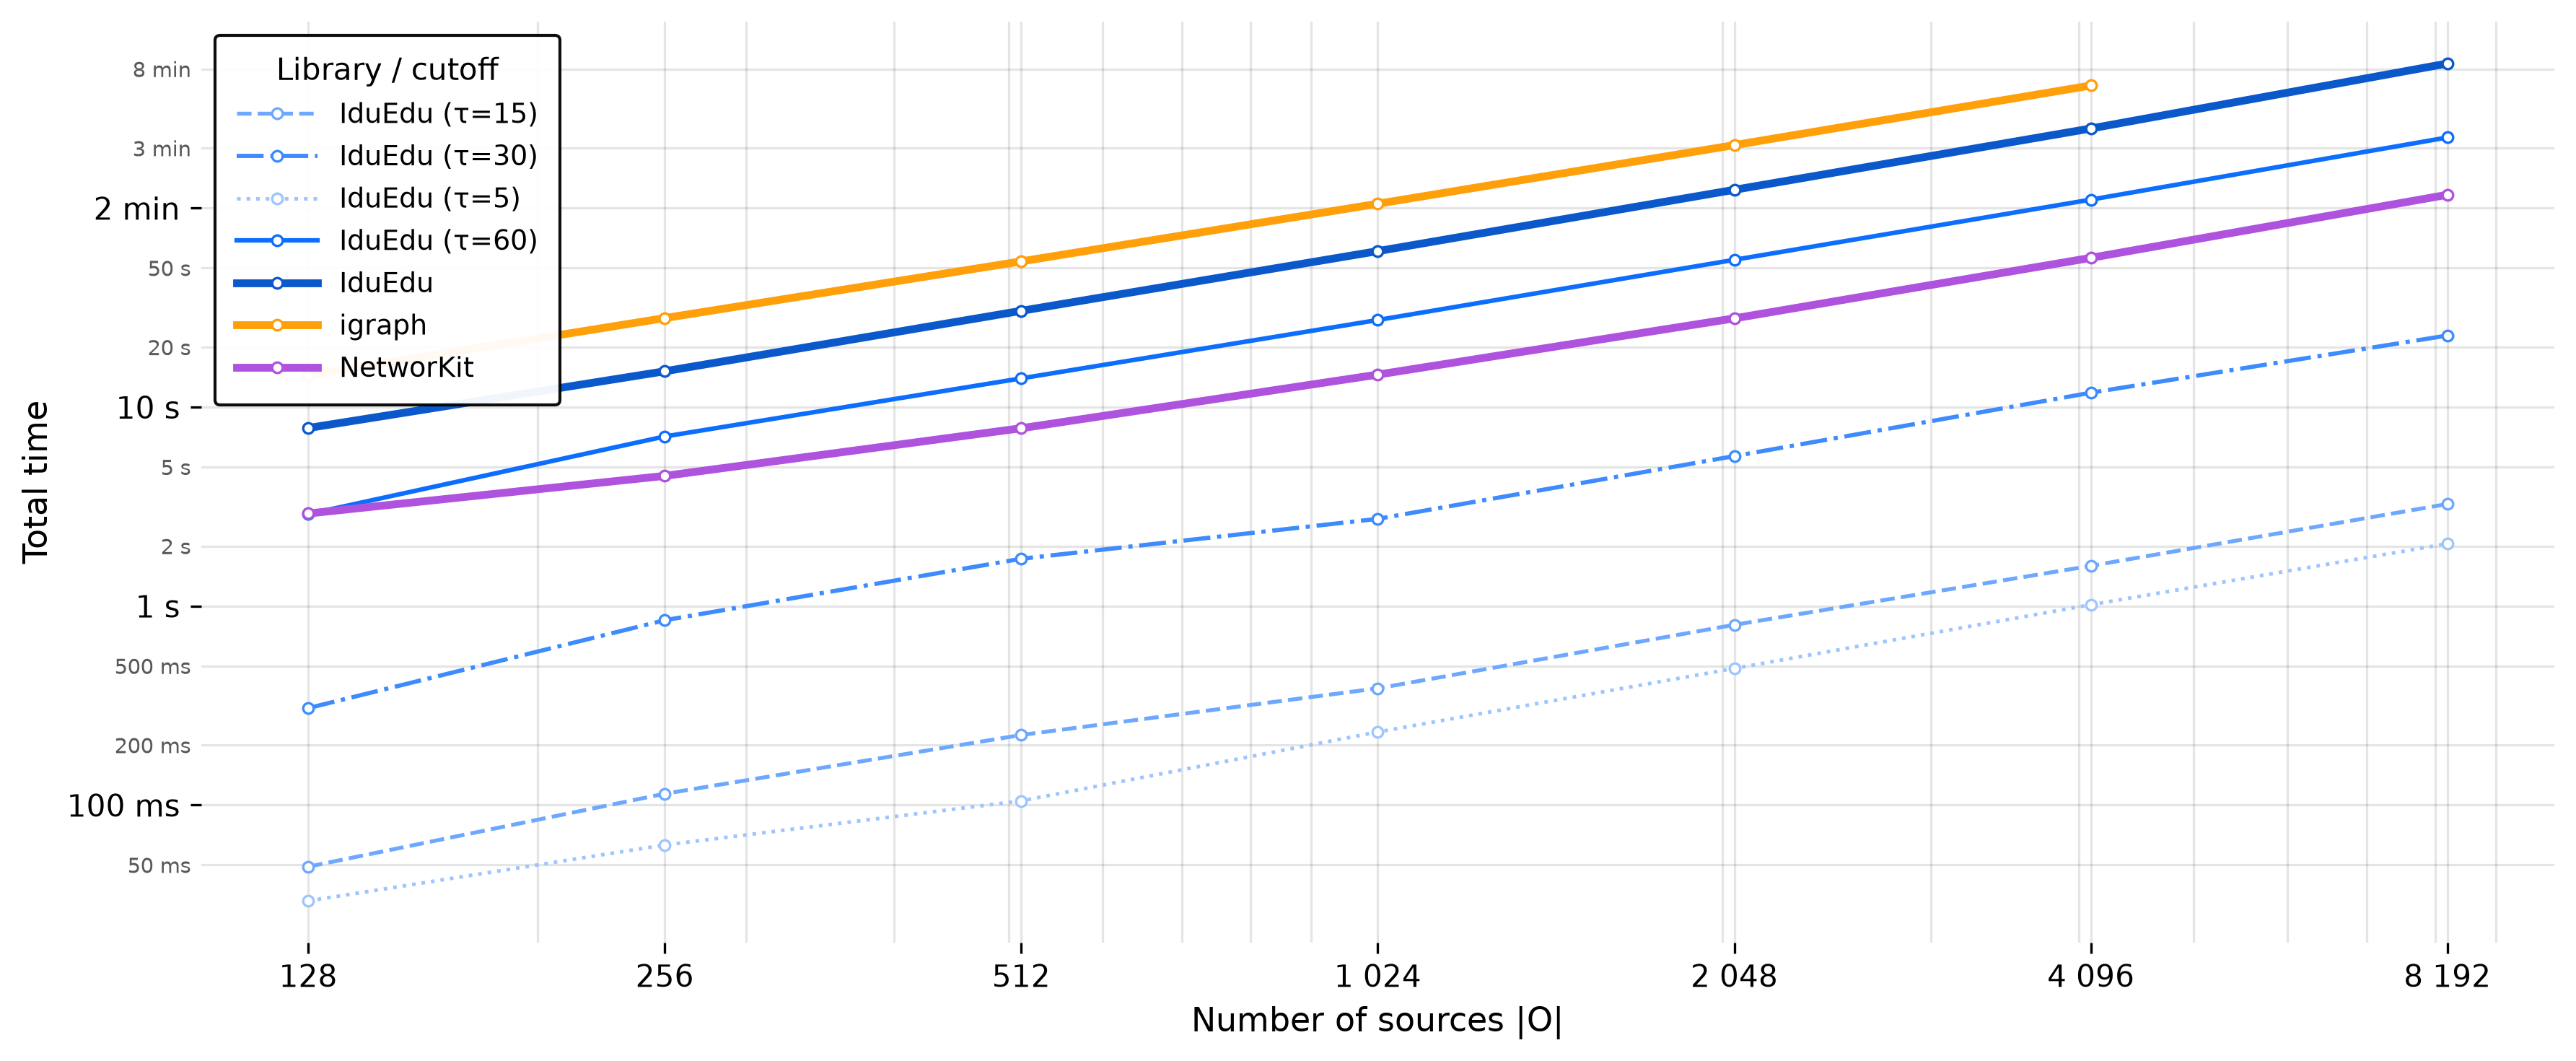
\includegraphics[width=\linewidth]{figures/od_time_square}
        \caption{Время вычисления квадратных OD-матриц (origins $\rightarrow$ origins)
            для IduEdu, NetworKit и igraph. Показано влияние порога отсечки на масштабируемость вычислений при росте числа источников.}
        \label{fig:od_time_square}
        \Description{OD matrix computation time for square origin-origin settings,
            highlighting the effect of cutoff thresholds on scalability.}
    \end{figure}

    В силу практических ограничений по времени выполнения igraph использовался только для $|O| < 8{,}192$, NetworKit — для $|O| < 65{,}536$.
    Замеры IduEdu выполнялись для всех рассматриваемых размерностей.

    \subsection{Summary for Experimental Evaluation}
    \label{subsec:summary-for-experimental-evaluation}
    В совокупности результаты показывают, что IduEdu сокращает время построения уличных графов относительно OSMnx при сопоставимых
    настройках и многократно выигрывает по памяти, сохраняя при этом эквивалентность результатов эталонным реализациям.
    В задачах вычисления OD-матриц адаптивные решения (разворот графа, временная отсечка) в сочетании с отсутствием этапа конвертации
    позволяют IduEdu быть конкурентоспособным с NetworKit и igraph, а в прямоугольных и cutoff-сценариях — превосходить их при росте размерности задачи.
    Таким образом, IduEdu покрывает полный цикл — от извлечения данных OpenStreetMap до масштабируемого расчёта метрик доступности — в рамках единого инструмента.


    \section{Ablation Studies}
    \label{sec:ablation-studies}

    Цель абляционных экспериментов — изолированно оценить вклад ключевых проектных решений IduEdu в вычислительную эффективность pipeline.
    Рассматриваются три механизма: (i) упрощение уличного графа на этапе построения, (ii) введение порога отсечки при вычислении
    OD-матриц и (iii) адаптивный разворот графа при несбалансированных множествах источников и назначений.

    \subsection{Graph Simplification}
    \label{subsec:graph-simplification}

    Упрощение уличного графа устраняет промежуточные вершины, не соответствующие функциональным узлам сети, и объединяет последовательности коллинеарных рёбер.
    Это приводит к сокращению числа вершин и рёбер без изменения топологии сети и без потери геометрической информации, необходимой для дальнейших расчётов.

    Абляция проводится путём сравнения времени построения пешеходных и автомобильных графов в IduEdu с включённым и отключённым упрощением.
    Для каждого города измеряется медианное время построения графа, итоговое число рёбер и детерминированный объём памяти результирующих таблиц графа.

    Результаты, представленные на рис.~\ref{fig:graph_simplification}, показывают, что эффект \texttt{simplify} не является универсальным и зависит от топологии сети.
    В пешеходной сети плотная структура пересечений и большое число локальных геометрических стыков делают пространственное
    объединение рёбер дорогим этапом: для таких графов дешевле быстро сформировать таблицы рёбер без предварительного упрощения.
    При этом упрощённый пешеходный граф остаётся существенно компактнее — упрощение сокращает число рёбер примерно в $2$--$3$ раза
    и во столько же уменьшает объём памяти результирующего представления.

    Для автомобильной сети картина обратная: топология обычно содержит больше протяжённых линейных участков и меньше мелких
    пешеходных пересечений, поэтому объединение геометрий быстрее окупается уже на этапе сборки.
    В этом режиме \texttt{simplify} одновременно сокращает число рёбер и уменьшает время построения графа.
    Следовательно, упрощение следует трактовать не как безусловное ускорение сборки, а как топологически зависимый обмен
    между стоимостью геометрического объединения и размером получаемого графа.

    С практической точки зрения это означает, что для сценариев с массовыми последующими расчётами упрощение остаётся
    важным этапом подготовки данных: даже когда оно увеличивает время построения пешеходного графа, выигрыш по размеру
    графа снижает потребление памяти и стоимость дальнейших алгоритмов поиска кратчайших путей (разд.~\ref{subsec:od_benchmark}).
    Для одноразовой сборки без последующих тяжёлых вычислений отключение упрощения может быть рациональным выбором.


    \begin{figure}[htb]
        \centering
        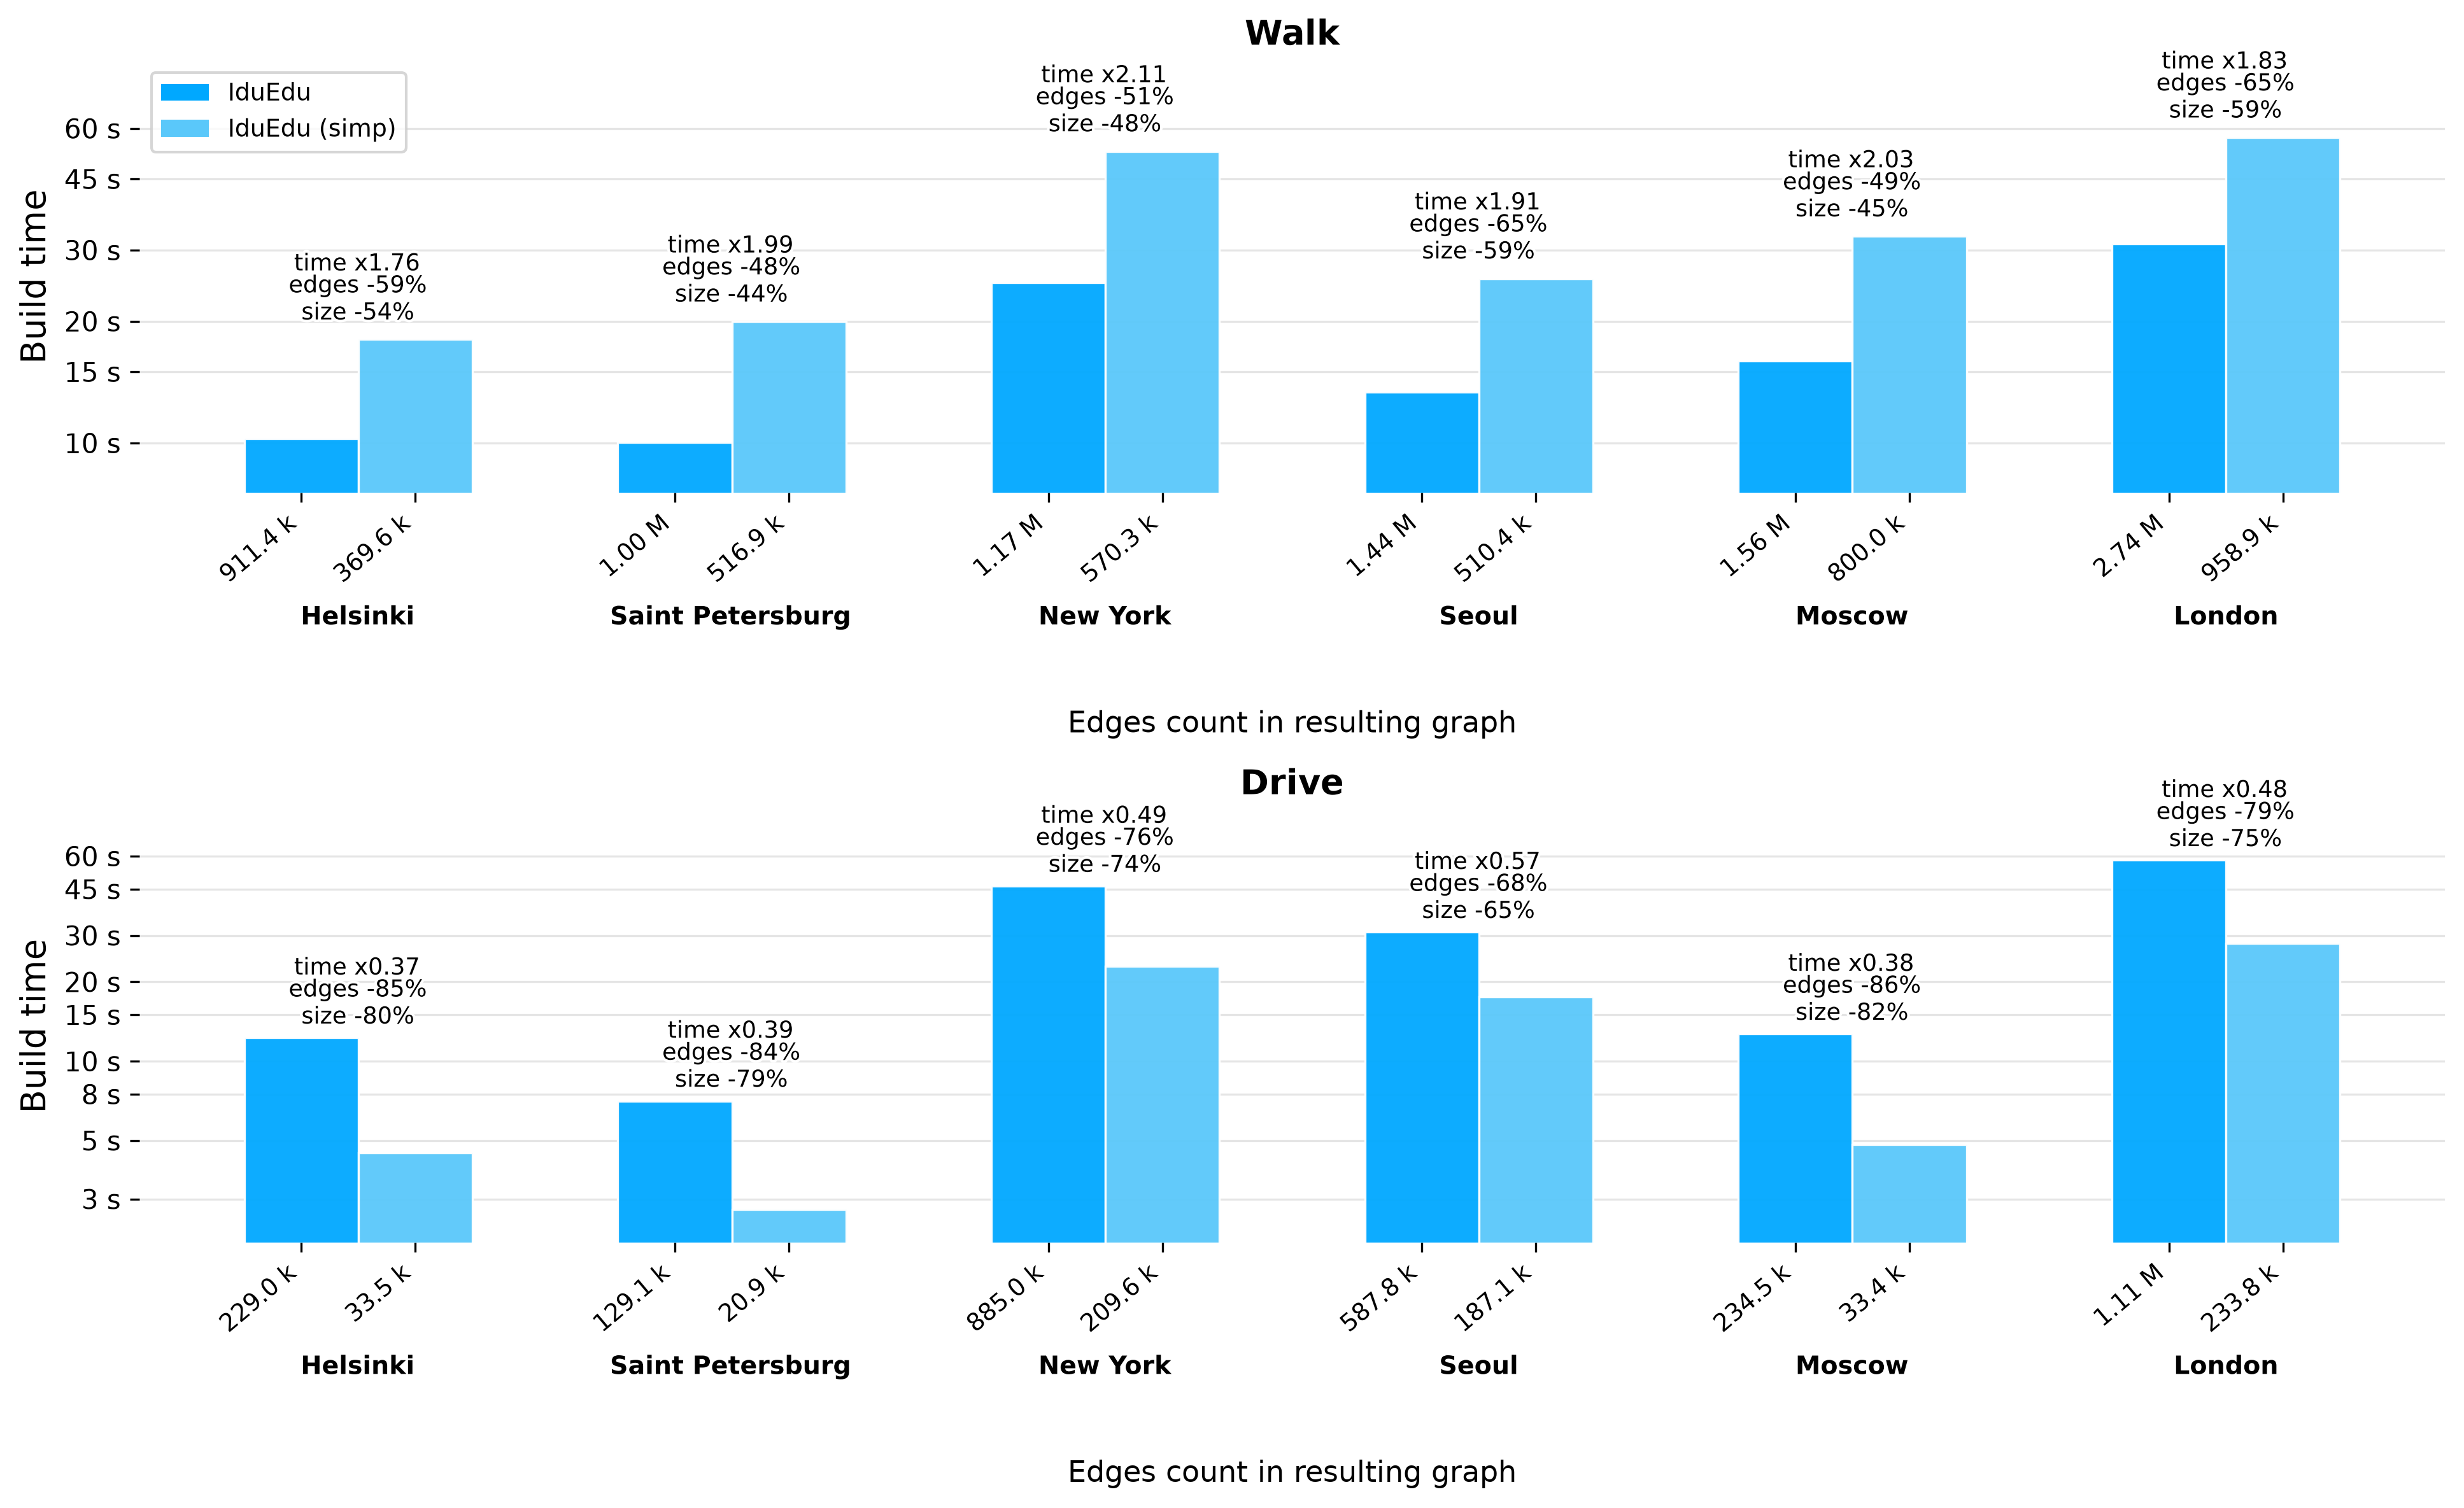
\includegraphics[width=\linewidth]{figures/ablation_simplify}
        \caption{Влияние упрощения графа на время построения пешеходных и автомобильных сетей в IduEdu.
        Под столбцами указано число рёбер в результирующем графе, а над группами столбцов — относительное изменение
        времени сборки, числа рёбер и памяти результирующего графа при включении упрощения.}
        \label{fig:graph_simplification}
        \Description{Bar chart comparing walk and drive graph build times in IduEdu with and without graph simplification across multiple cities.
        Each city is represented by two bars showing build time, annotated with the resulting number of edges.
        Text annotations indicate relative changes in build time, edge count, and graph memory under simplification.}
    \end{figure}

    \subsection{Cutoff in OD Matrix Computation}
    \label{subsec:cutoff-in-od-matrix-computation}

    Порог отсечки по длине пути ограничивает область поиска алгоритма кратчайших путей и позволяет вычислять разреженные OD-матрицы, ориентированные на задачи доступности.
    Абляция выполняется путём сравнения полного расчёта OD-матриц и расчёта с различными значениями порога времени пути~$\tau$.

    Эксперименты с квадратными OD-матрицами ($|O| = |D|$) показывают, что введение отсечки приводит к существенному
    снижению вычислительных затрат по мере роста размерности задачи (табл.~\ref{tab:od_cutoff_square}).
    В режиме полного расчёта время выполнения определяется глобальной структурой графа и глубиной обхода,
    тогда как использование cutoff локализует поиск в пространственной окрестности источников и ограничивает количество посещаемых вершин.

    Наибольший выигрыш наблюдается при малых значениях порога ($\tau = 5$–$15$ мин) и больших размерах матрицы.
    Так, уже при $|O| = 8{,}192$ относительное ускорение достигает $259\times$ по сравнению с полным расчётом.
    По мере увеличения порога отсечки эффект ослабевает: при $\tau = 60$ мин ускорение достигает $2\times$ даже для крупных матриц,
    что отражает приближение вычислений к полному обходу графа.

    Таким образом, использование cutoff наиболее эффективно в сценариях локальной доступности, типичных для пешеходного
    и транспортного анализа, где интерес представляет достижимость в ограниченном временном радиусе.

    \begin{table}
        \centering
        \caption{Relative speed-up of OD matrix computation in IduEdu with cutoff $\tau$
            for square OD matrices ($|O|=|D|$), measured against the full computation without cutoff.}
        \label{tab:od_cutoff_square}
        \small
        \begin{tabular}{lrrrrrrr}
            \toprule
            $\tau$ (min) & 128    & 256    & 512    & 1024   & 2048   & 4096   & 8192   \\
            \midrule
            5            & 237.88 & 240.25 & 290.16 & 260.95 & 254.33 & 247.33 & 258.85 \\
            15           & 160.20 & 132.77 & 135.41 & 157.52 & 153.55 & 157.74 & 163.59 \\
            30           & 25.57  & 17.83  & 17.62  & 22.16  & 21.80  & 21.27  & 23.27  \\
            60           & 2.71   & 2.13   & 2.18   & 2.22   & 2.25   & 2.28   & 2.35   \\
            \bottomrule
        \end{tabular}
    \end{table}

    \subsection{Adaptive Graph Reversal}
    \label{subsec:adaptive-graph-reversal}

    Адаптивный разворот графа используется при вычислении прямоугольных OD-матриц в случаях, когда число источников превышает число назначений.
    Поскольку один запуск алгоритма Дейкстры вычисляет кратчайшие пути до всех достижимых вершин, вычисление OD-матрицы
    между множествами мощностей $|O|$ и $|D|$ требует $\min(|O|,|D|)$ запусков алгоритма.

    Результаты эксперимента B3 (рис.~\ref{fig:od_time_rect}) показывают, что при $|O| \gg |D|$ разворот графа
    стабилизирует время вычислений IduEdu: с ростом $|O|$ при фиксированном $|D|=911$ число запусков алгоритма
    определяется меньшим множеством ($\min(|O|,|D|)=|D|$), и кривая времени практически выходит на плато,
    тогда как у NetworKit и igraph без разворота число запусков растёт вместе с $|O|$, и время продолжает увеличиваться.
    Этот эффект по построению отсутствует в квадратных OD-матрицах ($|O|=|D|$, рис.~\ref{fig:od_time_square}),
    где $\min(|O|,|D|)=|O|$, но играет ключевую роль для прямоугольных сценариев, типичных для задач оценки доступности.


    \section{Discussion \& Limitations}
    \label{sec:discussion-&-limitations}

    Предложенный в работе подход и реализованный в IduEdu pipeline ориентированы на воспроизводимые исследования городской мобильности,
    в которых требуется явное мультимодальное представление транспортной сети и масштабируемые вычисления метрик доступности.
    Полученные экспериментальные результаты показывают, что такой подход позволяет существенно снизить вычислительные
    затраты по сравнению с существующими решениями при работе с крупными городскими графами.
    Однако метод имеет ряд ограничений, которые важно учитывать при интерпретации результатов.

    Ключевым ограничением подхода является статическая модель общественного транспорта.
    Граф формируется на основе топологии маршрутов и остановочной инфраструктуры, извлечённых из OpenStreetMap, без учёта расписаний движения.
    Такое представление ориентировано на анализ структурной доступности и связности сети и не предназначено для точного моделирования временной динамики поездок.
    Кроме того, качество результирующего графа напрямую зависит от полноты и корректности открытых данных OSM\@.

    Вычислительные преимущества IduEdu во многом достигаются за счёт архитектурных решений: табличного представления
    графа с совпадающим вычислительным форматом, векторизованных операций при парсинге OSM, механизмов отсечки и разворота графа при расчёте матрицы.

    \section{Conclusion \& Future Work}
    \label{sec:conclusion-&-future-work}

    В данной работе был представлен IduEdu — Python-пайплайн для построения и анализа мультимодальных графов городской
    мобильности на основе открытых данных OpenStreetMap.
    В отличие от существующих инструментов, предложенный подход объединяет извлечение уличной сети, построение графа общественного транспорта,
    формирование мультимодального представления и расчёт метрик доступности в рамках единой формализации, опирающейся на табличное
    представление графа \texttt{UrbanGraph}, в котором пространственный и вычислительный форматы совпадают.
    Экспериментальная оценка на городских данных показывает, что такие архитектурные решения позволяют эффективно работать
    с крупными графами и большими наборами пространственных данных.

    В дальнейшем развитие IduEdu планируется в нескольких направлениях.
    Предполагается интеграция поддержки данных GTFS и возможность работы с временно-зависимыми графами общественного транспорта с учётом расписаний.
    Также возможно добавление различных методов маршрутизации и поиска путей в графах, что позволит применять IduEdu
    для более широкого класса задач пространственного и транспортного моделирования из коробки.

    %% \begin{acks}

    %% \end{acks}


    \bibliographystyle{ACM-Reference-Format}
    \bibliography{sample-base}


\end{document}
\endinput
